
The intensive use of generative programming techniques provides an elegant engineering solution to deal with the heterogeneity of platforms and technological stacks. The use of domain-specific languages for example, leads to the creation of numerous code generators that automatically translate high-level system specifications into multi-target executable code. 

Producing correct and efficient code generator is complex and error-prone. Although software designers provide generally high-level test suites to verify the functional outcome of generated code, it remains challenging and tedious to verify the behavior of produced code in terms of non-functional properties.

This chapter describes a black-box testing approach that automatically detect anomalies in code generators in terms of non-functional properties (i.e., resource usage and performance).
 
In fact, we adapt the idea of metamorphic testing to the problem of code generators testing.  Hence, our approach relies on the definition of high-level test oracles (i.e., metamorphic relations) to check the potential inefficient code generator among a family of code generators. 

We evaluate our approach by analyzing the performance of Haxe, a popular high-level programming language that involves a set of cross-platform code generators. 
%Experimental results show that our approach is able to detect some performance inconsistencies that reveal real issues in Haxe code generators.

This chapter is organized as follows: 

Section \ref{sec:cg_introduction} introduces the context of this work, i.e., the non-functional testing of code generators.

Section \ref{sec:cg_Motivation} presents the motivation and background of this work. In particular, we discuss in this section three motivation examples and the problems we are addressing.

Section \ref{sec:cd_approach} describes the general approach overview and the testing strategy.

In Section \ref{sec:cg_evaluation}, the evaluation and results of our experiments are discussed. Hence, we provide more details about the experimental settings, the code generators under test, the benchmark used, the evaluation metrics, etc. We discuss then the evaluation results.

Finally, we conclude in Section \ref{sec:cg-conclusion}. 


\section{Introduction}
\label{sec:cg_introduction}

Generative programming techniques become a common practice for software development to tame the runtime platform heterogeneity that exists in several domains such as mobile or Internet of Things development. 

The main benefit of using generative programming is to reduce the development and maintenance effort, allowing the development at a higher-level of abstraction through the use of Domain-Specific Languages (DSLs)~\cite{brambilla2012model} for example. 

DSLs, as opposed to general-purpose languages, are high level software languages that focus on specific problem domains. 
DSLs or models are generally coupled with the use of code generators that will automatically transform the manually designed models to software artifacts, which can be deployed on different target platforms. 

However, code generators are known to be very difficult to implement and maintain since they involve a set of complex and heterogeneous technologies~\cite{france2007model,guana2015developers}.

To preserve software reliability and quality, code generators have to respect different requirements. In fact, \textit{non-mature} code generators can generate defective software artifacts which range from uncompilable or semantically dysfunctional code that causes serious damage to the generated software; to non-functional bugs which lead to poor-quality code that can affect system reliability and performance (\eg, high resource usage, high execution time, etc.). 

As a matter of fact, these defects (or also anomalies) should be detected and corrected as early as possible in order to ensure the correct behavior of delivered software.

To check the correctness of the code generation process, developers often define (at design or runtime level) a set of test cases that will verify the functional behavior of generated code. 

After code generation, test suites are executed within each target platform, which may lead to either a correct behavior (\ie, expected output) or incorrect one (\ie, failures, errors).

However, the functional correctness of generated code is not enough to claim the effectiveness of code generators. Properties such as memory usage and performance are very important to evaluate. In some cases, the quality of the generated code can negatively influence on the non-functional requirements and cause performance issues\cite{hundt2011loop,ray2014large}.

Testing the non-functional properties of code generators is a challenging and time-consuming task because developers need to deploy and run code every time a change is made in order to analyze and verify its non-functional behavior.

This task becomes more tedious when targeting different platforms and software languages. Thus, different platform-specific tools will be needed to track bugs and identify the cause of execution failures~\cite{guana2014chaintracker,delgado2004taxonomy}. 

As stated in the state of the art, there is a lack of automatic solutions that check the non-functional issues such as the properties related to the resource consumption of generated code (Memory or CPU consumption).

%we propose a testing approach based on a runtime monitoring infrastructure to automatically check the potential inefficient code generators. This infrastructure, based on system containers as execution platforms, allows code-generator developers to evaluate the generated code performance. %In fact, we provide a fine-grained understanding of resource consumption and analysis of components behavior. 


In this chapter, we are presenting the following contributions:

\begin{itemize} 	
	
	\item We propose a fully automated black box testing approach for detecting code generator inconsistencies within code generator families. We use metamorphic relations as means of test oracles for our test suites. In this contribution, we focus on detecting anomalies related to performance and resource usage properties.
	
	\item We report the results of an empirical study by evaluating the non-functional properties of the Haxe code generators. 
	Haxe is a popular high-level programming language\footnote{\num{1442} GitHub stars} that involves a set of cross-platform code generators able to generate code to different target platforms. The obtained results provide evidence to support the claim that our proposed approach is able to detect code generator issues.
	

	
\end{itemize}

\section{Context and motivations}
\label{sec:cg_Motivation}

\subsection{Code generator families}
When confronted with the requirement to generate code for a wide range of languages, middleware, libraries, hardware architectures, and operating systems, different customizable code generators can be used to easily and efficiently  generate code for different platforms.

This work is based on the intuition that a code generator is often a member of a family of code generators\cite{chae2008building}.

\begin{mydef}[\textbf{Code generator family}]
	We define a code generator family as a set of code generators that takes as input the same language/model and generate code for different target platforms.
\end{mydef}
%Thus, we can automatically compare the performance between different versions
%of generated code (coming from the same source program). Based on this comparison, we can automatically detect singular resource consumptions that could reveal a code generator bug.

As motivating examples for this research work, we can cite three approaches that intensively develop and use code generator families: 
\paragraph{a. Haxe.} 	Haxe\footnote{\url{http://haxe.org/}}~\cite{dasnois2011haxe} is an open source toolkit for cross-platform development which compiles to a number of different programming platforms, including JavaScript, Flash, PHP, C++, C\#, and Java. Haxe involves many features: the Haxe language, multi-platform compilers, and different native libraries. The Haxe language is a high-level programming language which is strictly typed. This language supports both, functional and object-oriented programming paradigms. It has a common type hierarchy, making certain API available on every target platform. Moreover, Haxe comes with a set of code generators that translate manually-written code (in Haxe language) to different target languages and platforms.  
%Haxe code can be compiled for applications running on desktop, mobile, and web platforms. Compilers ensure the correctness of user code in terms of syntax and type safety. Haxe comes also with a set of standard libraries that can be used on all supported targets and platform-specific libraries for each of them. One of the main uses of Haxe is to develop cross-platform games or cross-platform libraries that can run on mobile, on the Web or on a Desktop.  
This project is popular (more than \num{1440} stars on GitHub).

\paragraph{b. ThingML.} ThingML\footnote{\url{http://thingml.org/}} is a modeling language for embedded and distributed systems~\cite{fleurey2011mde}. The idea of ThingML is to develop a practical model-driven software engineering tool-chain which targets resource-constrained embedded systems such as low-power sensors and microcontroller-based devices. ThingML is developed as a domain-specific modeling language which includes concepts to describe both software components and communication protocols. The formalism used is a combination of architecture models, state machines and an imperative action language. The ThingML tool-set provides a  code generator families  to translate ThingML to C, Java and JavaScript. It includes a set of variants for the C and JavaScript code generators to target different embedded systems and their constraints. 
This project is still confidential, but it is a good candidate to represent the modeling community practices.

\paragraph{c. TypeScript.} TypeScript\footnote{\url{https://www.typescriptlang.org/}}is a typed superset of JavaScript that compiles to plain JavaScript~\cite{rastogi2015safe}. In fact, it does not compile to only one version of JavaScript. It can transform TypeScript to EcmaScript 3, 5 or 6. It can generate JavaScript that uses different system modules ('none', 'commonjs', 'amd', 'system', 'umd', 'es6', or 'es2015')\footnote{Each of this variation point can target different code generators (function \textit{emitES6Module} vs \textit{emitUMDModule} in emitter.ts for example).}. 
This project is popular (more than \num{12619} stars on GitHub).

Functionally testing a code generator family in this case would be simple. Since the generated programs have the same input program, the oracle can be defined as the comparison between the functional outputs of these programs which should be the same.
In fact, based on the three sample projects presented above, we remark that all GitHub code repositories of the corresponding projects use unit tests to check the correctness of code generators.  

In terms of non-functional tests, we observe that ThingML and TypeScript do not provide any specific tests to check the consistency of code generators regarding the memory or CPU usage properties. Haxe provides two test cases\footnote{https://github.com/HaxeFoundation/haxe/tree/development/tests/benchs} to benchmark the resulting generated code. One serves to benchmark an example in which object allocations are deliberately (over) used to measure how memory access/GC mixes with numeric processing in different target languages. The second test evaluates the network speed across different target platforms.


\subsection{Issues when testing a code generator family}

The main difficulties with testing the resource usage properties of code generators is that we cannot just observe the execution of produced code, but we have to observe and compare the execution of generated programs with equivalent (or reference) implementations (i.e., in other languages). Even if there is no explicit oracle to detect inconsistencies for a single code generator, we could benefit from the family of code generators to compare the behavior of several generated programs and detect singular resource consumption profiles that could reveal a code generator inconsistency~\cite{hundt2011loop}. 

As a consequence, we define a code generator inconsistency as:

\begin{mydef}[\textbf{code generator inconsistency}]
	
	A code generator that produces code which has a singular behavior in terms of performance or resource usage compared to all equivalent implementations in the same family.
\end{mydef}

The potential issues that can result in code generator inconsistencies can be resumed as following:
\begin{itemize}
	\setlength\itemsep{0em}
	\item  the lack of use of a \textbf{specific function that exists in the standard library} of the target API language  that can speed or reduce the memory consumption of the resulting program.
	\item the lack of use of \textbf{a specific type that exists in the standard library} of the target language  that can speed or reduce the memory consumption of the resulting program.
	\item  the lack of use of\textbf{ a specific language feature in a target language} that can speed or reduce the memory consumption of the resulting program. 
\end{itemize}

Next section discusses the common process used by developers to automatically test the performance of generated code. We also illustrate how we can benefit from the code generators families to identify suspect singular behaviors.


%In short, then, we believe that testing the non-functional properties of code generators remains challenging and time-consuming task because developers have to analyze and verify code for each target platform using platform-dependent tools which makes the task of maintaining code generators very tedious. The heterogeneity of platforms and the diversity of target software languages increase the need of supporting tools that can evaluate the consistency and coherence of generated code regarding the non-functional properties. This paper describes a new approach, based on micro-services as execution platforms, to automate and ease the non-functional testing of code generators. This runtime monitoring infrastructure provides a fine-grained understanding of resource consumption and analysis of generated code's behavior.

\section{The traditional process for non-functional testing of a code generator family}
A reliable and acceptable way to increase the confidence in the correctness of a code generator family is to validate and check the functionality of generated code, which is a common practice for compiler validation and testing~\cite{jorges2014back,stuermer2007systematic,sturmer2005overview}.
%Therefore, developers try to check the syntactic and semantic correctness of the generated code by means of different techniques such as static analysis, test suites, etc., and ensure that the code is behaving correctly.  
However, proving that the generated code is functionally correct is not enough to claim the effectiveness of the code generator under test. 

In fact, code generators have to respect different requirements to preserve software reliability and quality~\cite{demertzi2011analyzing}. 
In this case, ensuring the code quality of generated code requires examining several non-functional properties such as code size, resource or energy consuption, execution time, etc~\cite{pan2006fast}.
A \textit{non-mature} code generator might generate defective software artifacts (code smells) that violates common software engineering practices, resulting in a poor-quality code that can affect system reliability and performance (e.g., high resource usage, high execution time, etc.).


Figure \ref{fig:bbackground.pdf} summarizes the classical steps required to ensure the code generation and non-functional testing of produced code from design time to runtime. 
We distinguish four major steps: the software design using high-level system specifications, code generation by means of code generators, code execution, and non-functional testing of generated code. 


\begin{figure*}[t]
	\center
	
	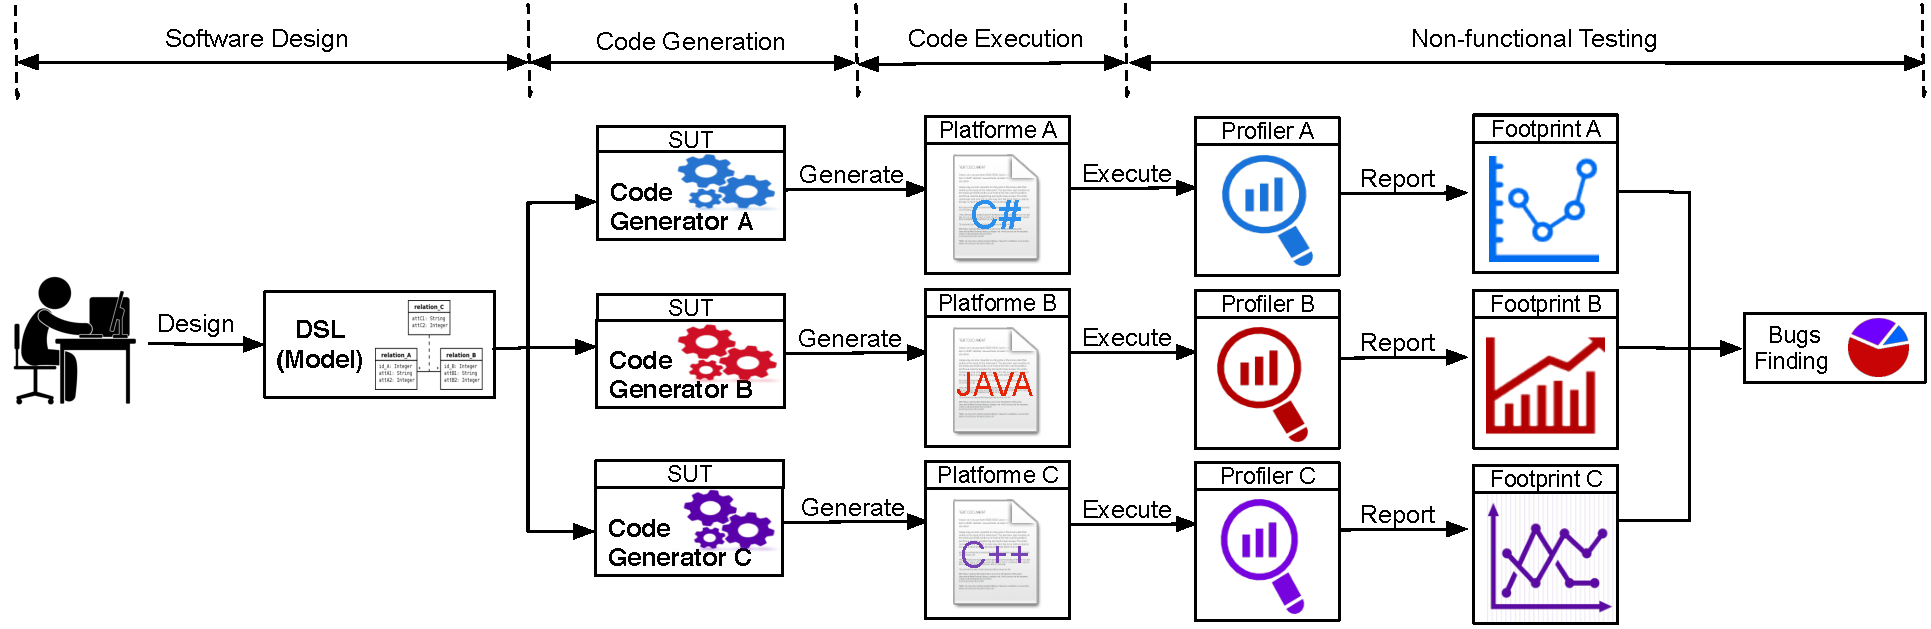
\includegraphics[width=1.\linewidth]{chapitre4/fig/background.pdf}
	\caption{An overall overview of the different processes involved to ensure the code generation and non-functional testing of produced code from design time to runtime: the classical way}
	\label{fig:bbackground.pdf}
\end{figure*}


In the first step, software developers have to define, at design time, the software's behavior using a high-level abstract language (DSLs, models, program, etc). Afterwards, developers can use platform-specific code generators to ease the software development and automatically generate code for different languages and platforms. We depict, as an example in Figure \ref{fig:bbackground.pdf}, three code generators from the same family capable to generate code to three software programming languages (JAVA, C\# and C++). The first step is to generate code from the previously designed model.
% Transformations from model to code within each code generator might be different and may integrate different transformation rules. As an example, we distinguish model-to-model transformations languages such as ATL~\cite{jouault2005transforming} and template-based model-to-text transformation languages such as Acceleo~\cite{musset2006acceleo} to translate high-level system specifications into executable code and scripts~\cite{bragancca2008transformation,czarnecki2003classification}. The main task of code generators is to transform models to general-purpose and platform-dependent languages.
Afterwards, generated software artifacts (e.g., JAVA, C\#, C++, etc.) are compiled, deployed and executed across different target platforms (e.g., Android, ARM/Linux, JVM, x86/Linux, etc.). 
%Thus, several code compilers are needed to transform source code to machine code (binaries) in order to get executed. 
Finally, to perform the non-functional testing of generated code, developers have to collect, visualize and compare information about the performance and efficiency of running code across the different platforms. 
Therefore, they generally use several platform-specific profilers, trackers, instrumenting and monitoring tools in order to find some inconsistencies or bugs during code execution~\cite{guana2014chaintracker,delgado2004taxonomy}. Finding inconsistencies within code generators involves analyzing and inspecting the code and that, for each execution platform. For example, one way to handle that, is to analyze the memory footprint of software execution and find memory leaks~\cite{nethercote2007valgrind}. Developers can then inspect the generated code and find some fragments of the code-base that have triggered this issue. %Such non-functional error could occur when the code generator produces code that presents for example: incorrect typing, faulty memory management, code-smells, etc. 
Therefore, software testers generally use to report statistics about the performance of generated code in order to fix, refactor, and optimize the code generation process. Compared to this classical testing approach, our proposed work seeks to automate the last three steps: generate code, execute it on top of different platforms, and find code generator inconsistencies. 


\section{Approach overview}
\label{sec:cd_approach}
Now, we describe our approach overview. Our contributions in this work are divided in two parts:
\begin{itemize}
	\item First, we describe our testing infrastructure for the automatic code generation deployment and monitoring. This work is presented in more details in Chapter \ref{chap:docker}. This contribution addresses the problem of software diversity and hardware heterogeneity, as discussed in Chapter \ref{chap:background}.
	
	\item Second, we present a methodology for automatically detecting inconsistencies in a code generator family. This approach addresses the oracle problem when testing the resource usage and performance properties.
\end{itemize}


\subsection{An infrastructure for non-functional testing using system containers}
\label{sec:cg-An infrastructure for non-functional testing using system containers}
In this contribution, we focus on evaluating the non-functional properties related to the resource usage and performance of generated code. To do so, many system configurations (i.e., execution environments, libraries, compilers, etc.) must be taken into account to efficiently generate and test code. 

However, tunning different applications (i.e., generated code) with different configurations on one single machine is complex. A single system has limited resources and this can lead to performance regressions. Moreover, each execution environment comes with a collection of appropriate tools such as compilers, code generators, debuggers, profilers, etc. Therefore, we need to deploy the test harness, i.e., the produced binaries, on an elastic infrastructure that provide facilities to the code generator developers to ensure the deployment and monitoring of generated code in different environment settings. 
Consequently, the testing infrastructure should provide support to automatically:
\begin{enumerate}
	\item Deploy the generated code, its dependencies and its execution environments
	\item Execute the produced binaries in an isolated environment 
	\item Monitor the execution 
	\item Gather performance metrics (CPU, Memory, etc.)
\end{enumerate}

To ensure these four main steps, we rely on system containers~\cite{soltesz2007container} as a dynamic and customizable execution environment for running and evaluating the generated programs in terms of resource usage.

\begin{figure*}[h]
	\center
	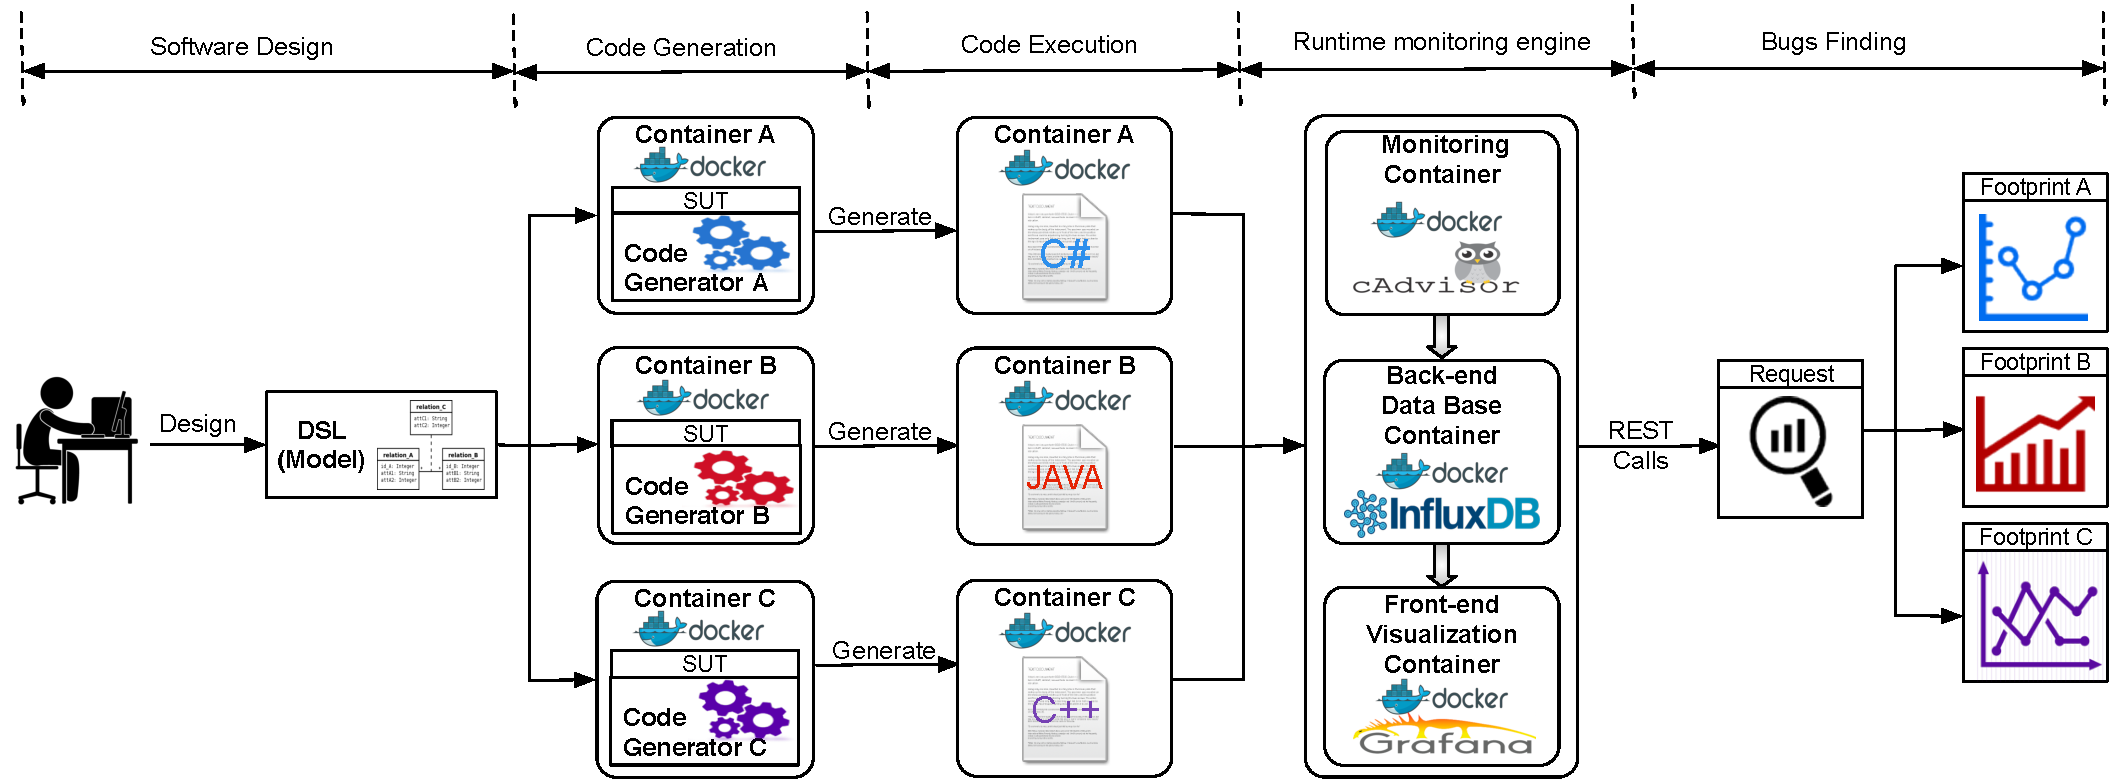
\includegraphics[width=1.\linewidth]{chapitre5/fig/docker_background2.pdf}
	\caption{A technical overview of the different processes involved to ensure the code generation and non-functional testing of produced code from design time to runtime.}
	\label{fig:cg-infra}
\end{figure*}

Figure \ref{fig:cg-infra} shows the new container-based infrastructure used for testing code generators. Compared to the classical method presented in Figure \ref{fig:bbackground.pdf}, we added the following features: 
\begin{itemize}
	\item[--] At the code generation level: Code generators are configured inside different containers in order to generate code for the target platform.
	\item[--] At the code execution: Libraries, compilers and different dependencies are configured in different containers in order to execute the generated code. For each target platform a new instance is created.
	\item[--] At the non-functional level: We add a runtime monitoring engine (based on containers) in order to extract the resource usage properties.
\end{itemize}

Chapter \ref{chap:docker} provides more details about the technical choices we have made to synthesize this testing infrastructure.




\subsection{A metamorphic testing method for automatic detection of code generators inconsistencies}
Automatically detecting non-functional issues in code generators raises the oracle problem since there is no a clear definition of how the oracle might be defined and how we can determine the expected outcomes of selected test cases.

We discussed in section \ref{sec:cg-Summary: oracle definition approaches} of Chapter \ref{chap:SOTA} several approaches from the software testing community to alleviate the oracle problem. Among the attractive approaches that can be applied to test code generators, we distinguish the metamorphic testing approach (derived oracles). This approach is already applied for generators, especially for testing compilers\cite{donaldson2016metamorphic,tao2010automatic,le2014compiler}. In the following, we describe the basic concept of metamorphic testing and our adaptation of this testing approach to test the code generator families in terms of resource usage and performance.

\subsubsection{Basic concept of metamorphic testing}
In this section, we shall introduce the basic concept of metamorphic testing (MT). 
MT, proposed by Chen et al. \cite{chen1998metamorphic}, is a technique conceived to alleviate the oracle problem. It is based on the idea that often it is simpler to understand the relation between test cases' outputs rather than reasoning about the relation between test inputs and outputs. 

MT recommends that, given one or more test cases (called "source test cases", "original test cases", or "successful test cases") and their expected outcomes (obtained through multiple executions of the target program under test), one or more follow-up test cases can be constructed to verify the necessary properties (called "metamorphic relations" or "MRs") of the system or function to be implemented. In this case, the generation of the follow-up test cases and verification of the test results require the respect of the MR.

The classical example of MT is that of a program that computes the \textit{sin} function. A useful metamorphic relation for \textit{sin} functions is $\textit{sin(x) = sin($\pi$ - x)}$. Thus, even though the expected value for the source test case \textit{sin(50)} for example in not known, a follow-up test case can be constructed to verify the MR defined earlier. In this case, the follow-up test case is $\textit{sin($\pi$ - 50)}$ which must produce an output value that is equal to the one produced by the original test case \textit{sin(50)}. If this property is violated, then a failure is immediately detected.
MT generates follow-up test cases as long as the metamorphic relations are respected.
This is an example of a metamorphic relation: an input transformation that can be used to generate new test cases from existing test data, and an output relation (MR), that compares the outputs produced by a pair of test cases.

MR can be any properties involving the inputs and outputs of two or more executions of the target program such as equalities, inequalities, periodicity properties, convergence constraints, subsumption relationships and many others. 

Because MT checks the relations among several executions rather than the correctness of individual outputs, MT can be used to fully automate the testing process without any manual intervention. 
However, constructing metamorphic relations is typically a manual task that demands thorough knowledge of the program under test. It also depends on the application context and domain. 
The effectiveness of metamorphic testing is highly dependent on the specific metamorphic relations that are used, and designing effective metamorphic relations is thus a critical step when applying metamorphic testing.

We describe in the next section our adaptation of MT to the problem of non-functional testing of code generators families.

\subsubsection{Application of MT to the non-functional testing of code generator families}
In general, MT can be applied to any problem in which a necessary property involving multiple executions of the target function can be formulated. Some examples of successful applications are presented in \cite{zhou2004metamorphic}. They includes the testing of simulation programs; the testing of numerical programs such as those for solving partial differential equations; the testing of graphics-rendering programs; and testing compilers.

To apply MT, there are four basic steps to follow:

\begin{enumerate}
 \item Find the properties of the system under test: the system should be investigated manually in order to find intended MRs defining the relation between inputs and outputs. This is based on the source test cases.
 \item Generate/select test inputs that satisfy the MR: this means that new follow-up test cases must be generated or selected in order to verify their outputs using the MR.
 \item Execute the system with the inputs and get outputs: original and follow-up test cases are executed in order to gather their outputs.
 \item Check whether these outputs satisfy the MR, and if not, report failures.
\end{enumerate}

We develop now these four points in details in order show our MT adaptation to the code generators testing problem. 
\subsubsection[(Step 1)]{Metamorphic relation }

Step 1 consists in identifying necessary properties of the program under test and represent them as metamorphic relations among multiple test case inputs and their expected outputs.

In the context of code generators testing, we apply the concept of metamorphic testing described above to detect inconsistencies that violate MRs.
To do so, we have to define suitable MRs to automate this process.

As already stated, a metamorphic relation is a relation between different executions.
If we use the MR definition as presented in \cite{tao2010automatic,chan2006integration}:

\begin{mydef}[\textbf{Metamorphic relation}]

Let $(x_{1}, x_{2},..., x_{k})$ be a series of inputs to a function $f$, where $k$ $\geqslant$ 1, and $(f(x_{1}, x_{2},..., x_{k})$ be the corresponding series of results. Suppose $(f(x_{i1}), f(x_{i2}),..., f(x_{im}))$ is a subseries, possibly an empty subseries, of $(f(x_{1})$, $f(x_{2})$,..., $f(x_{k}))$. Let $(x_{k+1}, x_{k+2},..., x_{n})$ be another series of inputs to $f$, where $n \geqslant k+1$, and $(f(x_{k+1})$, $f(x_{k+2})$,..., $f(x_{xn}))$ be the corresponding series of results. Suppose, further, that there exists relations $r(x_{1}$, $x_{2}$,..., $x_{k}$, $f(x_{i1})$, $f(x_{i2})$,...., $f(x_{im})$, $x_{k+1}$, $x_{k+2}$,..., $x_{n}))$ and $r'$$(x_{1}$, $x_{2}$,..., $x_{n}$, $f(x_{1}$, $f(x_{2}$,..., $f(x_{n}))$ such that $r'$ must be true whenever $r$ is satisfied. We say that 


\textbf{MR} = {$(x_{1}, x_{2},...,x_{n}, f(x_{1}), f(x_{2}),..., f(x_{n}) \mid$

$r(x_{1}, x_{2},..., x_{k}, f(x_{i1}), f(x_{i2}),...., f(x_{im}), x_{k+1}, x_{k+2},..., x_{n}))$

$\Rightarrow r'(x_{1}, x_{2},..., x_{n}, f(x_{1}), f(x_{2}),..., f(x_{n}))$} 

is a metamorphic relation. When there is no ambiguity, we simply write the metamorphic relation as 	

\textbf{MR}: if $r(x_{1}, x_{2},..., x_{k}, f(x_{i1}), f(x_{i2}),...., f(x_{im}), x_{k+1}, x_{k+2},..., x_{n}))$

then $r'(x_{1}, x_{2},..., x_{n}, f(x_{1}), f(x_{2}),..., f(x_{n})).$

Furthermore, $x_{1}, x_{2},..., x_{k}$ are known as source test cases and $x_{k+1}, x_{k+2},..., x_{xn}$ are known as follow-up test cases
%Let (x1, x2,..., xk) be a series of inputs to a function f , where k > 1, and f(x1), f(x2),..., f(xk) be the corresponding series of results. Suppose f(xi1 ), f(xi2 ),..., f(xim ) is a subseries, possibly an empty subseries, of f(x1), f(x2),..., f(xk). Let xk+1, xk+2,..., xn be another series of inputs to f , where n ≥ k + 1, and f(xk+1), f(xk+2),..., f(xn) be the corresponding series of results. Suppose, further, that there exists relations r(x1, x2, ..., xk, f(xi1 ), f(xi2 ), ..., f(xim ), xk+1, xk+2, ..., xn) and r (x1, x2,..., xn, f(x1), f(x2),..., f(xn)) such that r must be true whenever r is satisfied. We say that MR = { (x1, x2,..., xn, f(x1), f(x2),..., f(xn)) | r(x1, x2,..., xk, f(xi1 ), f(xi2 ),..., f(xim ), xk+1, xk+2,..., xn) → r (x1, x2,..., xn, f(x1), f(x2),..., f(xn)) } is a metamorphic relation. When there is no ambiguity, we simply write the metamorphic relation as MR: If r(x1, x2,..., xk, f(xi1 ), f(xi2 ),..., f(xim ), xk+1, xk+2,..., xn) then r (x1, x2,..., xn, f(x1), f(x2),..., f(xn)). Furthermore, x1, x2, ..., xk are know

\end{mydef}

A code generator family can be looked as a function: $C : I \rightarrow P$, where $I$ is the domain of valid high-level source programs and $P$ is the domain of the target programs that are generated by the different code generators of the same family. The property of a code generator family implies that the generated programs $P$ share the same behavior as it is specified in $I$ using the high-level system specification. 


The availability of multiple generators with comparable functionality allow us to adapt MT in order to detect non-functional inconsistencies. In fact, if we can find out proper R relation of the non-functional behavior, we can get the metamorphic relation and conduct MT for testing code generator families.
Let $f(P(x))$ be a function that calculates a non-functional metric of a generated program $P$ (such as execution time or memory usage of $P$) for an input test suite denoted by $x$. Since we have different program versions generated in the same family, we denote by $(P_{1}(x)$, $P_{2}(x)$,..., $P_{n}(x))$ the set of generated programs. The corresponding outputs would be $(f(P_{1})$, $f(P_{2})$,..., $f(P_{n}))$. Thus, our MR looks like this:

\begin{equation}
	 R(P_{1}(x), P_{2}(x),..., P_{n}(x))  \Rightarrow R(f(P_{1}(x)), f(P_{2}(x)),..., f(P_{n}(x)))
\end{equation}

On the one hand, we use the following equation $P_{1}(x) \equiv P_{2}(x)$ to denote \textit{the functional equivalence relation} between two generated programs $P_{1}$ and $P_{2}$ from the same family. This means that the generated programs $P_{1}$ and $P_{2}$ have the same behavioral design, and for any test suite $x$, they have the same functional output. 
If this relation is not satisfied that means, that there is at least one faulty code generator that produced incorrect code. In this this work, we focus on the non-functional testing, so we ensure that this relation is ensured by excluding all the programs that do not exhibit the same behavior. 


On the other hand, since we are comparing equivalent implementations of the same program written in different languages, we assume that the memory usage and execution time should be more or less the same with a small variation for each test suite across the different versions. Obviously, we are expecting to get a variation between different executions because we are comparing the execution time and memory usage of test suites that are written in different languages and executed using different technologies (e.g., interpreters for PHP, JVM for JAVA, etc.). 
This observation is also based on initial experiments, where we evaluate the resource usage/execution time of several test suites across a set of equivalent versions generated using a code generator family (presented in details in the evaluation section \ref{sec:cg_evaluation}). As a consequence, we use the notation $\Delta\{f(P_{1}(x)), f(P_{2}(x))\}$ to designate the variation of memory usage or execution time of test suite execution $x$ across two version of generated code written in different languages $P_{1}$ and $P_{2}$. We suppose that this variation should note exceed a certain threshold value $T$, otherwise, we raise a code generator inconsistency.
Based on this intuition, the MR can be represented as:

\begin{equation}
P_{1}(x) \equiv P_{2}(x) \equiv ... \equiv P_{n}(x) \Rightarrow \Delta\{f(P_{1}(x)), f(P_{2}(x)),..., f(P_{n}(x))\} < T\quad (n\geqslant 2)
\end{equation}

This MR is equivalent to say that: \textbf{if} a set of functionally equivalent programs are generated using the same code generator family $((P_{1}(x)$, $P_{2}(x)$,...,$P_{n}(x))$, and with the same input parameters $x$ \textbf{then} the comparison of their non-functional outputs $(f(P_{1}(x))$, $f(P_{2}(x))$,..., $f(P_{n}(x)))$ should be the same while taking into account a tolerance interval defined by the variation $\Delta$ that may not exceed a specific threshold value $T$.

The generated code that violates this metamorphic property represents an inconsistency and its corresponding code generator is considered as defective.

 



\subsubsection[(Steps 2, 3, and 4)]{Metamorphic testing}
\label{sec:cg-Metamorphic testing}
\begin{figure}[h]
	\centering
	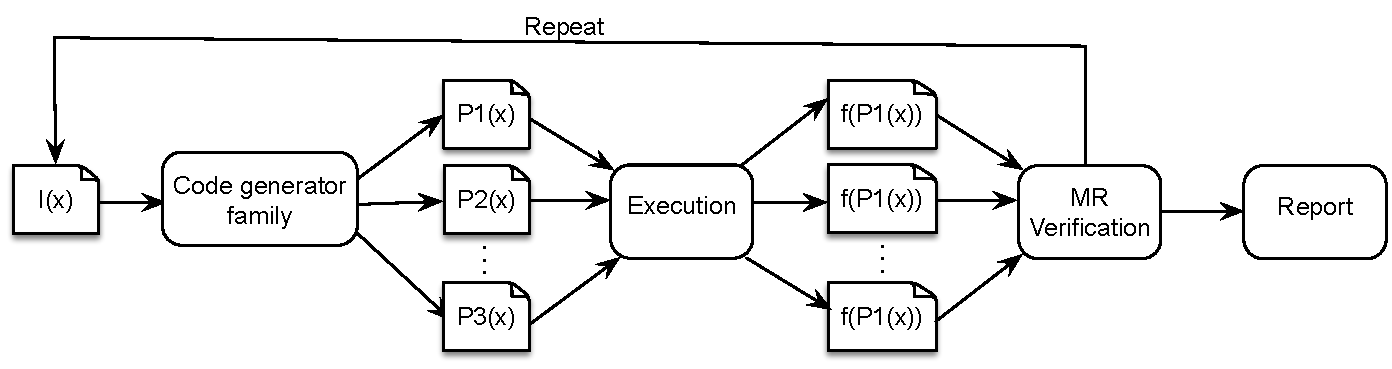
\includegraphics[width=1.\linewidth]{chapitre4/fig/MT}
	\caption{The metamorphic testing approach for automatic detection of code generator inconsistencies}
	\label{fig:cg_MT}
\end{figure}

So far, we have defined the metamorphic property (MR) necessary for inconsistencies detection. We describe now our automatic metamorphic testing approach based on this relation (steps 2, 3, and 4). 
Figure \ref{fig:cg_MT} shows the approach overview.
The code generator family takes the same input program I and generate a set of equivalent test programs $(P_{1}$, $P_{2}$,...,$P_{n})$. Test suites are also automatically generated since we suppose that they are created at design time. In fact, the same test suite (test cases + input data values) is passed to all generated programs. This corresponds to step 2 where new follow-up test cases must be generated or selected in order to verify their outputs using the MR. 
Then, generated programs and their corresponding test suites are executed (step 3). Afterwards, we measure the memory usage or execution time of these generated programs $(f(P_{1}(x))$, $f(P_{2}(x))$,..., $f(P_{n}(x)))$. Finally, the execution results are compared and verified using the MR defined earlier (step 4).
In this process, inconsistencies will be reported when we detect singular performance behavior of one running test suites for a specific target.





\subsubsection{Variation threshold}
\label{sec:cg-Variation threshold}
One of the main question that may be raised when applying our MT approach is how can we find the right variation threshold $T$ from which an inconsistency is detected? Answering this question is very important to prove the effectiveness of our MT approach.

To do so, we conduct a statistical analysis of the non-functional outputs of original test inputs in order to find an accurate threshold value $T$ and then, detect inconsistencies using follow-up test inputs.
 
Before that, the non-functional outputs need to be prepared to make them suitable for the statistical techniques employed by our methodology. Thus, we describe first our process for data preparation:

\paragraph{Data preparation}~\\ 
As depicted in Table \ref{tab:Non-functional output results}, each program comes with a set of test suites $(t_{1}$, $t_{2}$,..., $t_{m})$. Evaluating a test suite requires the calculation of the memory usage or execution time $f(P_{1}(t_{i}))$,  $f(P_{2}(t_{i}))$,..., $f(P_{n}(t_{i}))$ where $(1 \leq i \leq m)$  across all target software platforms. Thus, obtained results represent a matrix where columns indicate the non-functional value (raw data) for each target software platform and rows indicate the corresponding test suite.
\begin{table}[h]
	\centering
	
	\begin{tabular}{|c| c |c |c| c|}				
		\hline

		 &  Target platform $1$ &  Target platform $2$ & ... & Target platform $n$  \\ \hline
		$t_{1}$  &  $f(P_{1}(t_{1}))$ &  $f(P_{2}(t_{1}))$ & ... & $f(P_{n}(t_{1}))$  \\ \hline
		$t_{2}$ &  $f(P_{1}(t_{2}))$ &  $f(P_{2}(t_{2}))$ & ... & $f(P_{n}(t_{2}))$  \\ \hline
		... &  ... &  ... & ... & ...  \\ \hline
		$t_{m}$ &  $f(P_{1}(t_{m}))$ &  $f(P_{2}(t_{m}))$ & ... & $f(P_{n}(t_{m}))$  \\ \hline
	\end{tabular}
	
	\caption{Non-functional output results}
	\label{tab:Non-functional output results}
\end{table}
The non-functional data should be converted into a format that is understood by our statistical methods. One way to compare these non-functional outputs is to study the factor differences. In other words, we would evaluate for each target platform the number of times (the factor) that a test suite takes to run compared to a reference test suite. The reference test suite in our case is the minimum obtained non-functional value across the n target platforms. The resulting factor is the ratio between the actual non-functional value and the minimum value obtained among the n versions. The following equation is applied for each cell in order to transform our data:

\begin{equation}
F(f(P_{j}(t_{i})))=\frac{f(P_{j}(t_{i}))}{Min(f(P_{1}(t_{i})),..., f(P_{n}(t_{i})))}  
\end{equation}

The reference value will get a factor value $F = 1$ corresponding to the minimum value among the n targets. The maximum value is the one leading to the maximum deviation for the reference test suite. For example, let $P_{1}$ be the generated program in Java. If the execution time needed to run $t_{1}$ yields to the minimum value $f(P_{1}(t_{1}))$ compared to other versions, then $f(P_{1}(t_{1}))$ will get a factor value $F$ equal to $1$ and the other versions will be divided by $f(P_{1}(t_{1}))$ to get the corresponding factor values compared to Java.

Next step is to automatically detect the large deviations, we describe then, our statistical approaches.

\paragraph{Statistical analysis}~\\
 
In our MT approach, an inconsistency is a performance deviation corresponding to the extreme variation values.
We propose two methods to automatically detect these inconsistencies: Principal components analysis (PCA) and R charts (R-chart).\\
Table \ref{tab:Statistical methods} gives an overview of these two statistical methods.
\begin{table}[h]
	\centering
	
	\begin{tabular}{|l| l |l |}				
		\hline
		
		\textbf{Type} &  \textbf{Technique} &  \textbf{Method}    \\ \hline
		Input sensitive  &  R-chart &  Define T as an upper control limit  \\ \hline
		Input insensitive &  PCA &  The Mahalanobis distance used to define the T \\ \hline
	\end{tabular}
	
	\caption{Non-functional output results}
	\label{tab:Statistical methods}
\end{table}

\subparagraph{R-Chart}~\\
In this approach, the automatic variation detection between the different versions of code is determined by comparing the non-functional measurements based on a statistical quality control technique called \textit{R-Chart} or \textit{range chart}. 
R-Chart is used to analyze variation within processes. It is designed to detect changes in variation over time and to evaluate the consistency of process variation.
R-Chart uses control limits to represent the limits of variation that should be expected from a process. LCL denotes the Lower Control Limit and UCL denotes the Upper Control Limits UCL.
 
When a process is within the controlled limits, any variation is normal. It is said that the process is \textbf{in control}. 
Outside limit variations, however, considered as deviations and the R-chart is considered as \textbf{out of control} which means that the process variation is not stable. Thus, It tells that there is an inconsistency leading to this high variation deviation (see Figure \ref{fig:cg-rechart})

In our case, a process represents the $n$ non-functional outputs obtained after the execution of a test suite $t_{i}$. As we defined the metamorphic relation, this variation within a single process have to be lower than a threshold $T$. In our settings, this variation must be between the LCL and UCL.

\begin{figure}[h]
	\centering
	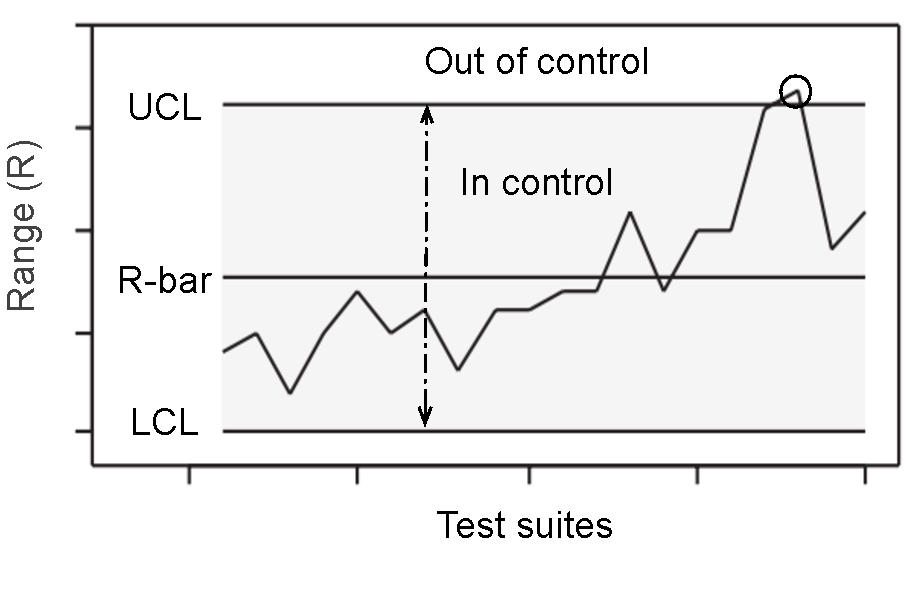
\includegraphics[width=0.6\linewidth]{chapitre4/fig/rchat}
	\caption{The R-Chart process}
	\label{fig:cg-rechart}
\end{figure}

Therefore, for each process we calculate the range $R$ corresponding to the difference between the maximum and minimum non-functional outputs for each test suite across all target platforms:

\begin{equation}
R(t_{i})= Max(f(P_{1}(t_{i})),..., f(P_{n}(t_{i}))) - Min(f(P_{1}(t_{i})),..., f(P_{n}(t_{i})))  
\end{equation}
The R displays change in the within process dispersion to quantify the variation of executing the same test suite $t_{i}$ across different versions of the program under test.
To determine whether the process is in control or not, we need to determine the control limits values. UCL and LCL reflect the actual amount of variation that is observed. Both, are a function of R-bar ($\bar{R}$). $\bar{R}$ is the average of R across all processes (test suites).
The UCL and LCL are calculated as follows:
\begin{equation}
\begin{split} 
UCL = D_{4}\bar{R}\\
LCL = D_{3}\bar{R}
\end{split} 
\label{eqUCL}
\end{equation}
where $D_{4}$, $D_{3}$, are control chart constants that depend on the number of variables inside each process. For example of a code generator family composed of five code generators, $D_{4}$ is equal to and $D_{3}$ is equal to 0. 

From a MT perspective, the UCL represents the threshold $T$ value from which we detect a high variation deviation, leading to an inconsistency. As we stated earlier, the UCL is a function of $\bar{R}$, and $\bar{R}$ is a function of range differences. So, the UCL value is sensitive to new generated follow-up test suites. In order to evaluate the MR for new generated test suites, the UCL (or $T$) value is updated and the variation is evaluated with the new threshold value. 

We present in the following another statistical approach that is input insensitive and can find a general threshold value to define variation limit.





%\subparagraph{title} 


\subparagraph{PCA}~\\

With a large number of program versions, the non-functional data matrix (Table \ref{tab:Non-functional output results}) may be too large to study and interpret the variation properly. There would be too many pairwise correlations between the different versions to consider and the variation is impossible to display (graphically) when test suites are executed in more than three target platforms.
With 12 variables, for example, there will be more than 200 three-dimensional scatter plots to be designed to study the variation and correlations.
To interpret the data in a more meaningful form, it is therefore necessary to reduce the number of variables composing our data.

Principal Component Analysis\footnote{\url{https://en.wikipedia.org/wiki/Principal_component_analysis}} (PCA) is a multivariate statistical approach that uses an orthogonal transformation to convert a set of observations of possibly correlated variables into a set of values of linearly uncorrelated variables called Principal Components (PC). It can be applied when data are collected on a large number of variables from a single population. Thus, we apply the PCA approach to our case study because our dimension space as it is presented in Table\ref{tab:Non-functional output results}, is composed of a set of processes (test suites) where $n$ variables (e.g., target programming languages) are composing each observation. The variability within our model is correlated to these $n$ variables representing the test suites running on $n$ target platforms. 

The main objective of PCA is to reduce the dimensionality of the original data and explain the maximum amount of variance with the fewest number of principal components. To do so, PCA is concerned with summarizing the variance-covariance matrix. It involves computing the eigenvectors and eigenvalues of the variance-covariance matrix. The eigenvectors are used to project the data from $p$ dimensions down to a lower dimensional representation. The eigenvalues give the variance of the data in the direction of the eigenvector. The first eigenvector is the vector which defines the direction of maximumn variance in the data.

The first principal component is calculated such that it accounts for the greatest possible variance in the data set. The second principal component is calculated in the same way, with the condition that it is uncorrelated with (i.e., perpendicular to) the first principal component and that it accounts for the next highest variance. The eigenvector associated with the largest eigenvalue has the same direction as the first principal component. The eigenvector associated with the second largest eigenvalue determines the direction of the second principal component.

PCA use many data transformations and statistical concepts. We are not interested in studying all the mathematical aspects of PCA. Thus, we use an existing R package\footnote{\url{http://factominer.free.fr/}} to transform and reduce our data into two PCs in order to visualize the variation of all our data points in a 2-dimensional space.

Our intuition behind the PCA approach is to conduct an extreme-value analysis in order to find data points at the boundaries of multivariate data. These extreme points represent, from a statistical perspective, \textit{outliers}. Following our MT approach, these points correspond to the inconsistencies (or deviation) we would detect. 

Outliers have an important influence over the PCs. An outlier is defined as an observation which does not follow the model followed by the majority of the data.
One way to detect outliers is to use a metric called Score Distance (SD). SD measures the outlyingness of the observations within the PCA space. It thus measures how far an observation lies from the rest of the data within the PCA subspace. 
SD measures the statistical distance from a PC score to the center of the scores. For an observation $x_{i}$ the  score distance is defined as:
\begin{equation}
SD_{i}=\sqrt{\sum_{j=1}^{a} \frac{t_{ij}^{2}}{\lambda_{j}}}
\end{equation}
where $a$ is the number of PCs forming the PCA space, $t_{ij}$ are the elements of the score matrix obtained after running PCA, and $\lambda_{j}$ is the variance of the $j$th PC which corresponds to the $j$th eigenvalue.

In order to find the outliers, we compute the 97.5\%-Quantile Q of the Chi-square distribution as a cutoff value of the SD ($\sqrt{\chi_{a,0.975}^{2} }$). It corresponds to an ellipse that covers 97.5\% of the data points and this forms a confidence ellipse.
Any samples whose SD are larger than the cutoff are identified as the outliers. This cut-off represents the variation threshold $T$ we would define using this PCA approach.

%It is equal to the squared Mahalanobis distance from the model center to sample i within the score subspace.
%Cut-off values help to distinguish between outliers and regular observations. Any samples whose Mahalanobis distances are larger than the cutoff are identified as the outliers.
\begin{remark}
The R-chart method presented earlier, defines a dynamic threshold value (UCL) where follow-up test suites influence on this value. However, using PCA, we are able to analyze the non-functional data of original test suites in order to define a general threshold value (Cutoffs) which is steady. Thus, follow-up test suites that exceed this value, causing a high performance or resource usage deviation, are identified as inconsistencies (outliers).
\end{remark}

We move now to present the evaluation of our approach.


\section{Evaluation}
\label{sec:cg_evaluation}
So far, we have presented an automated approach for detecting inconsistencies within code generator families. So, we shape our goal as this research question:

\textbf{RQ1: } 
\textbf{\textit{How effective is our metamorphic testing approach for automatically detecting inconsistencies in code generator families?}} 

To answer this question, we evaluate the implementation of our approach by explaining the design of our empirical study and the different methods we used to assess the effectiveness of our approach. 
The experimental material is available for replication purposes\footnote{\url{https://testingcodegenerators.wordpress.com/}}.
\subsection{Experimental setup}
\subsubsection{Code generators under test: Haxe compilers}
In order to test the applicability of our approach, we conduct experiments on a popular high-level programming language called Haxe and its code generators. Haxe is an open source toolkit for cross-platform development which compiles to a number of different programming platforms, including JavaScript, Flash, PHP, C++, C\# and Java. Haxe involves many features: the Haxe language, multi-platform compilers, and different native libraries. 
The Haxe language is a high-level programming language which is strictly typed. This language supports both functional programming and object-oriented programming paradigms. It has a common type hierarchy, making certain API available on every targeted platform.
Haxe comes with a set of compilers that translate manually-written code (in Haxe language) to different target languages and platforms. 
Haxe code can be compiled for applications running on desktop, mobile and web platforms. It comes also with a set of standard libraries that can be used on all supported targets and platform-specific libraries for each of them.

The process of code transformation and generation can be described as following: Haxe compilers analyze the source code written in Haxe language. Then, the code is checked and parsed into a typed structure, resulting in a typed abstract syntax tree (AST). This AST is optimized and transformed afterwards to produce source code for the target platform/language.
Haxe offers the option of choosing which platform to target for each program using command-line options. Moreover, some optimizations and debugging information can be enabled through command-line interface, but in our experiments, we did not turn on any further options. 

The Haxe code generators constitute the code generator family we would evaluate in this work.

\subsubsection{Cross-platform benchmark}
One way to prove the effectiveness of our approach is to create benchmarks. Thus, we use the Haxe language and its code generators to build a cross-platform benchmark. The proposed benchmark is composed of a collection of cross-platform libraries that can be compiled to different targets. In these experiments, we consider a code generator family composed of five target Haxe compilers: Java, JS, C++, CS, and PHP code generators. To select cross-platform libraries, we explore github and we use the Haxe library repository\footnote{\url{http://thx-lib.org/}}. So, we select seven libraries that provide a set of test suites with high code coverage scores. 

In fact, each Haxe library comes with an API and a set of test suites. These tests, written in Haxe, represent a set of unit tests that covers the different functions of the API. The main task of these tests is to check the correct functional behavior of generated programs. To prepare our benchmark, we remove all the tests that fail to compile to our five targets (i.e., errors, crashes and failures) and we keep only test suites that are functionally correct in order to focus only on the non-functional properties.
Moreover, we add manually new test cases to some libraries in order to extend the number of test suites. The number of test suites depends on the number of existing functions within the Haxe library.

We use then these test suites to transform functional tests into stress tests. This can be useful to study the impact of this load on the resource usage properties of the five target versions. For example, if one test suite consumes a lot of resources for a specific target, then this could be explained by the fact that the code generator under test has produced code that is very greedy in terms of resources.
Thus, we run each test suite 1K times to get comparable values in terms of resource usage.
Table \ref{tab:Description of selected benchmark libraries} describes the Haxe libraries that we have selected in this benchmark to evaluate our
approach and the number of test suites used per benchmark.

\begin{table}[h]
	\centering
	
		\begin{tabular}{|c|c|p{8.5cm}|}				
			\hline
			\textbf{Library} & \textbf{\#TestSuites} & \textbf{Description} \\
			\hhline{|=|=|=|}
			Color  &  19 &  Color conversion from/to any color space   \\ \hline
			Core & 51  & Provides extensions to many types  \\ \hline
			Hxmath & 6  & A 2D/3D math library  \\ \hline
			Format  &  4 & Format library such as dates, number formats   \\ \hline
			Promise & 5  & Library for lightweight promises and futures  \\ \hline
			Culture & 5  & Localization library for Haxe \\ \hline
			Math & 5  & Generation of random values \\ \hline
		\end{tabular}
	
	\caption{Description of selected benchmark libraries}
	\label{tab:Description of selected benchmark libraries}
\end{table}

In total, we have 95 test suites to execute across all benchmark programs.
\subsubsection{Evaluation metrics used}
We use to evaluate the efficiency of generated code using the following non-functional metrics:

-\textit{Memory usage}:
It corresponds to the maximum memory consumption of the running test suite. Memory usage is measured in \SI{}{\mega\byte}

-\textit{Execution time}:
Program execution time is measured in seconds.

We recall that our testing infrastructure is able to evaluate other non-functional properties of generated code such as code generation time, compilation time, code size, CPU usage. We choose to focus, in this experiment, on the performance (i.e., execution time) and resource usage (i.e., memory usage).

\subsubsection{Setting up infrastructure}

To assess our approach, we configure our previously proposed container-based infrastructure in order to run experiments on the Haxe case study.
Figure \ref{fig:settingup.pdf} shows a big picture of the testing and monitoring infrastructure considered in these experiments.

\begin{figure}[h]
	\centering
	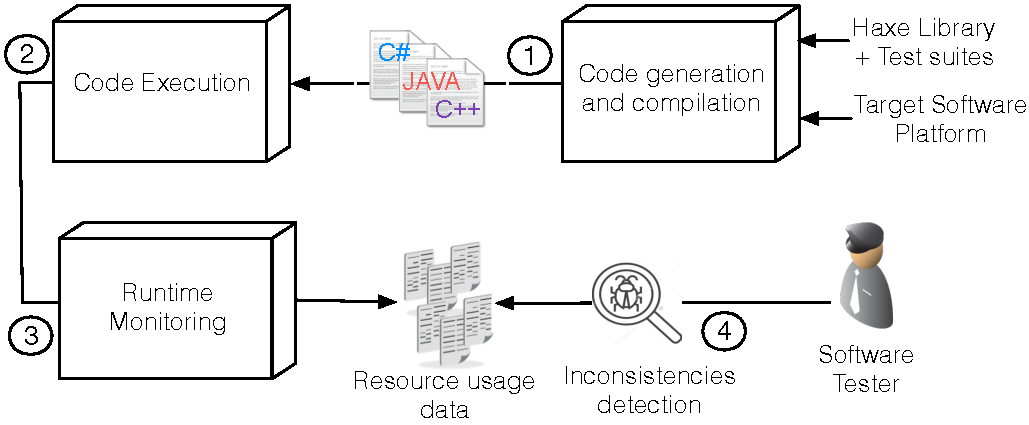
\includegraphics[width=0.8\linewidth]{chapitre4/fig/settingup.pdf}
	\caption{Infrastructure settings for running experiments}
	\label{fig:settingup.pdf}
\end{figure}

First, a first component is created in where we install the Haxe code generators and compilers. It takes as an input the Haxe library we would test and the list of test suites (step 1). It produces as an output the source code for specific software platforms. These files are saved in a shared repository call \textit{Data Volume}.

Afterwards, generated files are compiled (if needed) and automatically executed within the execution container (Step 2). This execution container is a pre-configured container instance where we install all the required execution environments such as php interpreter, NodeJS, etc. 

In the meantime, while running test suites inside the container, we collect runtime resource usage data using the components showed in step 3, 4, and 5 (presented in details in Chapter \ref{chap:docker}).

Finally, in step 6 we provide a mechanism to extract these resource usage metrics via http requests. In our experiment, we are gathering the maximum memory usage values without presenting the graphs of resource usage profiles.

To obtain comparable and reproducible results, we use the same hardware across all experiments: a farm of AMD A10-7700K APU Radeon(TM) R7 Graphics processor with 4 CPU cores (\SI{2.0}{\GHz}), running Linux with a 64 bit kernel and \SI{16}{\giga\byte} of system memory. We reserve one core and \SI{4}{\giga\byte} of memory for each running container. 

\subsection{Experimental methodology and results}
In the following paragraphs, we report the methodology we used to answer \textbf{RQ1} and results of our experiments. 

\subsubsection{Method}
We now conduct experiments based on the new created benchmark. 
The goal of running these experiments is to observe and compare the behavior of generated code in order to detect code generator inconsistencies.
%We recall, as mentioned in the motivation, that we are not using any oracle function to detect inconsistencies. However, we rely on the comparison results across different targets to detect code generator inconsistencies.

Therefore, we set up, first, our container-based infrastructure as it is presented in Section \ref{sec:cg-An infrastructure for non-functional testing using system containers} in order to generate, execute, and collect the resource usage metrics of our benchmark programs.
Afterwards, we prepare and scale our raw data to make it valuable for efficient statistical analysis. Then, we conduct the R-chart and PCA analysis as described in Section \ref{sec:cg-Variation threshold} in order to analyze the performance and resource usage variations. This we lead us to define an appropriate formula of our MR that is used to automatically detect inconsistencies within code generator families (Section \ref{sec:cg-Metamorphic testing}). Finally, we report the inconsistencies we have detected.


%as a quality metric, the standard deviation to quantify the amount of variation among execution traces (i.e., memory usage or execution time) and that, for the five target languages. We recall that the formula of standard deviation is the square root of the variance. Thus, we are calculating this variance as the squared differences from the mean. Our data values in our experiment represent the obtained values in five languages. So, for each test suite we are taking the mean of these five values in order to calculate the variance.
%A low standard deviation of a test suite execution, indicates that the data points (execution time or memory usage data) tend to be close to the mean which we consider as an acceptable behavior.  
%On the other hand, a high standard deviation indicates that one or more data points are spread out over a wider range of values which can be more likely interpreted as a code generator inconsistency. 

\subsubsection{Results}
\paragraph{R-chart results}~\\
\begin{figure}
	\centering  
	\subfigure[R-chart of the Core benchmark program]{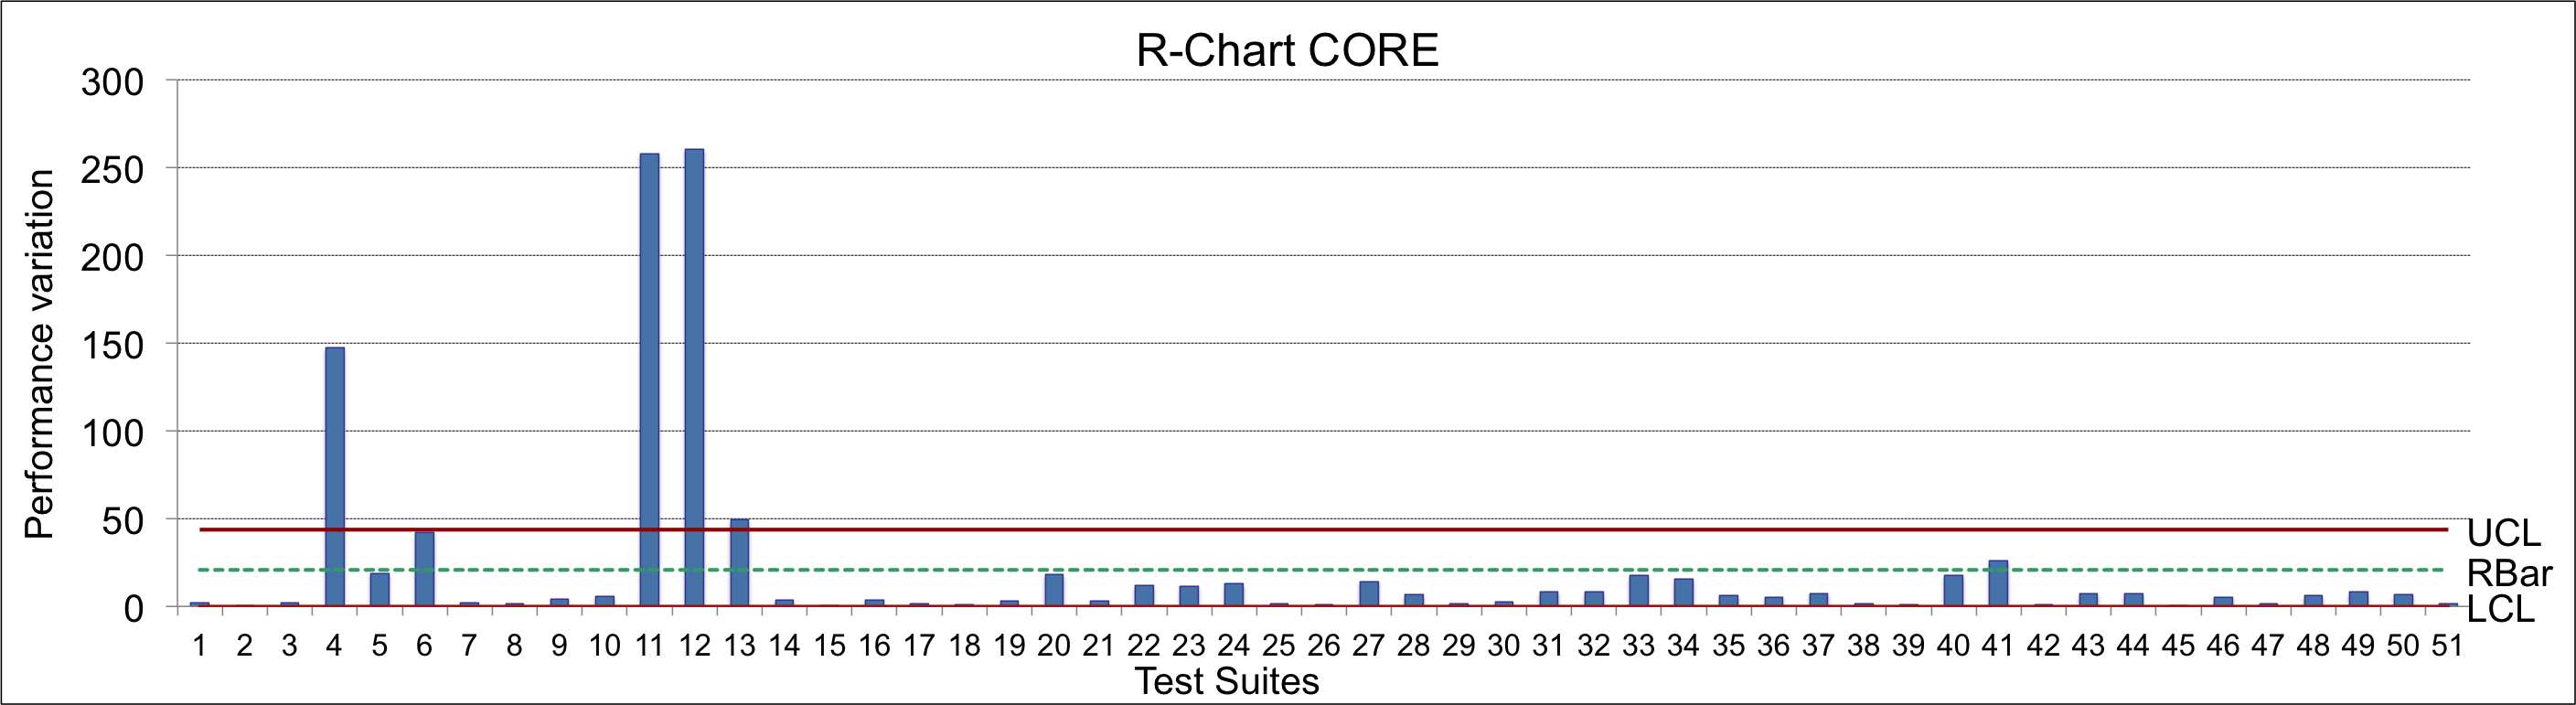
\includegraphics[width=0.96\linewidth]{chapitre4/fig/1.png}\label{rt1}}
	\subfigure[R-chart of the Color benchmark program]{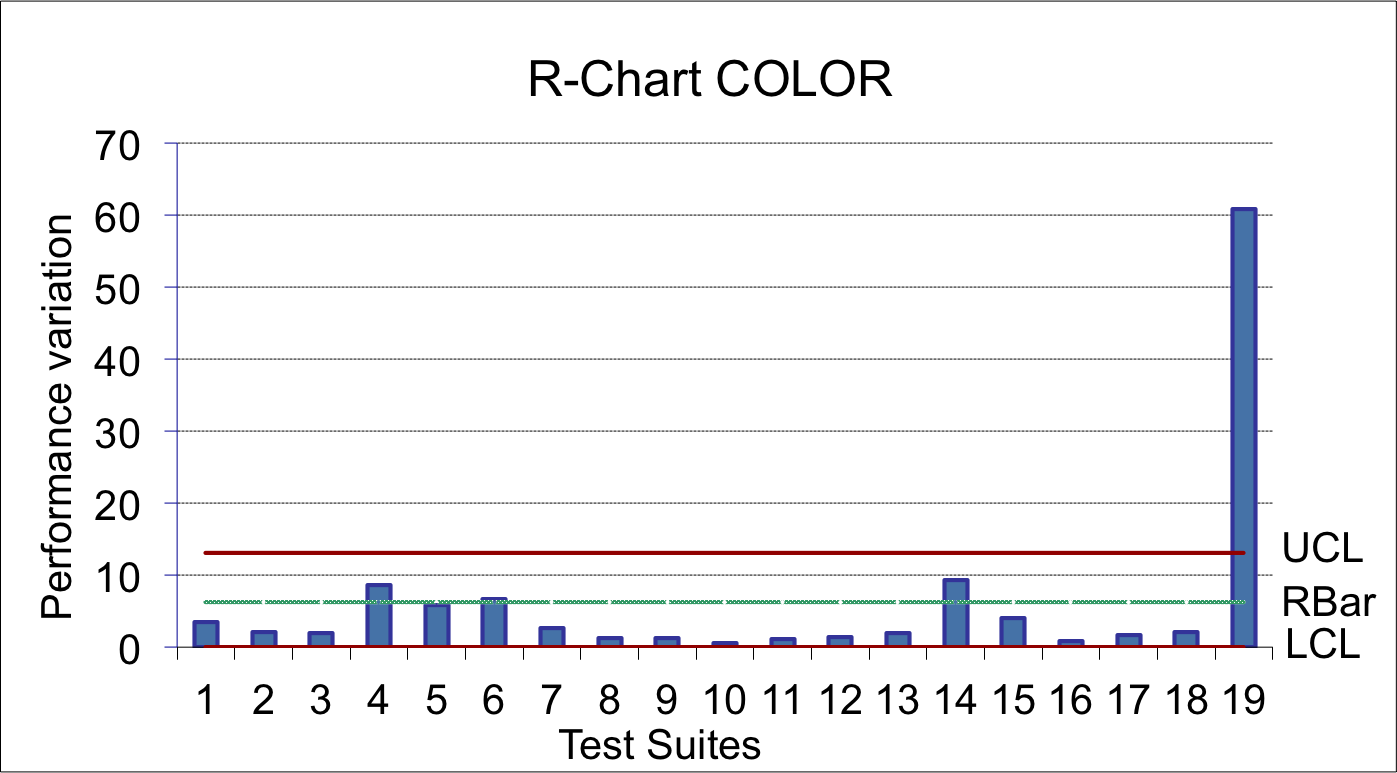
\includegraphics[width=0.48\linewidth]{chapitre4/fig/2.png}\label{rt2}}
	\subfigure[R-chart of the Hxmath benchmark program]{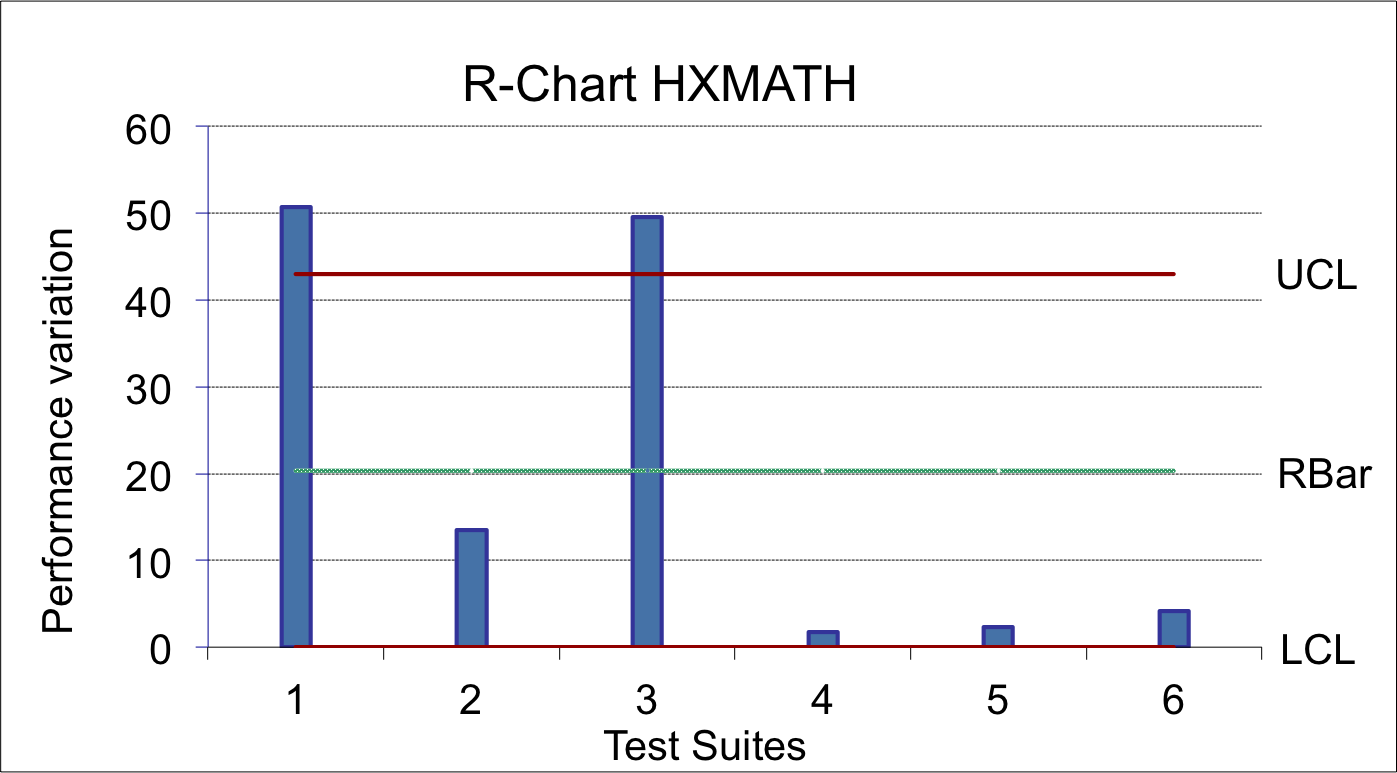
\includegraphics[width=0.48\linewidth]{chapitre4/fig/3.png}\label{rt3}}
	\subfigure[R-chart of the Format benchmark program]{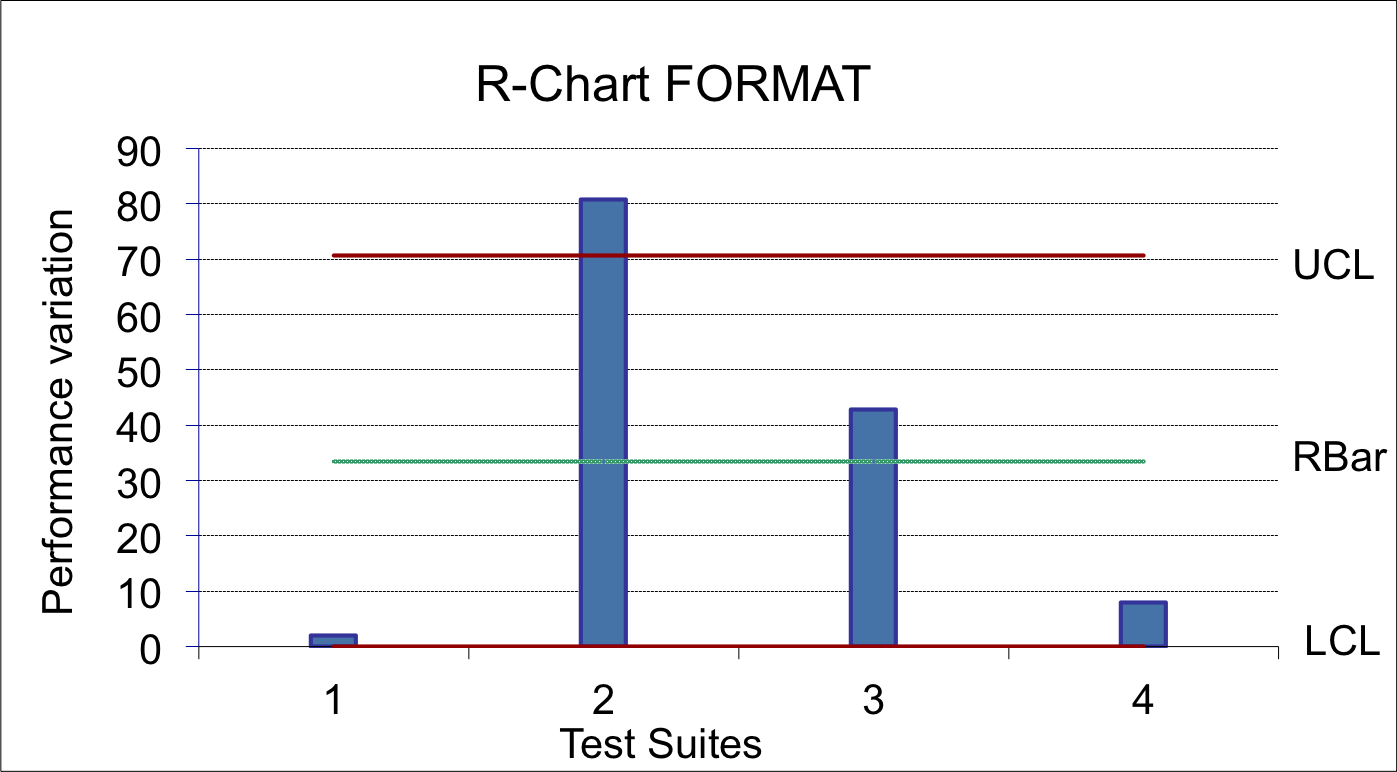
\includegraphics[width=0.48\linewidth]{chapitre4/fig/4.png}\label{rt4}}
	\subfigure[R-chart of the Promise benchmark program]{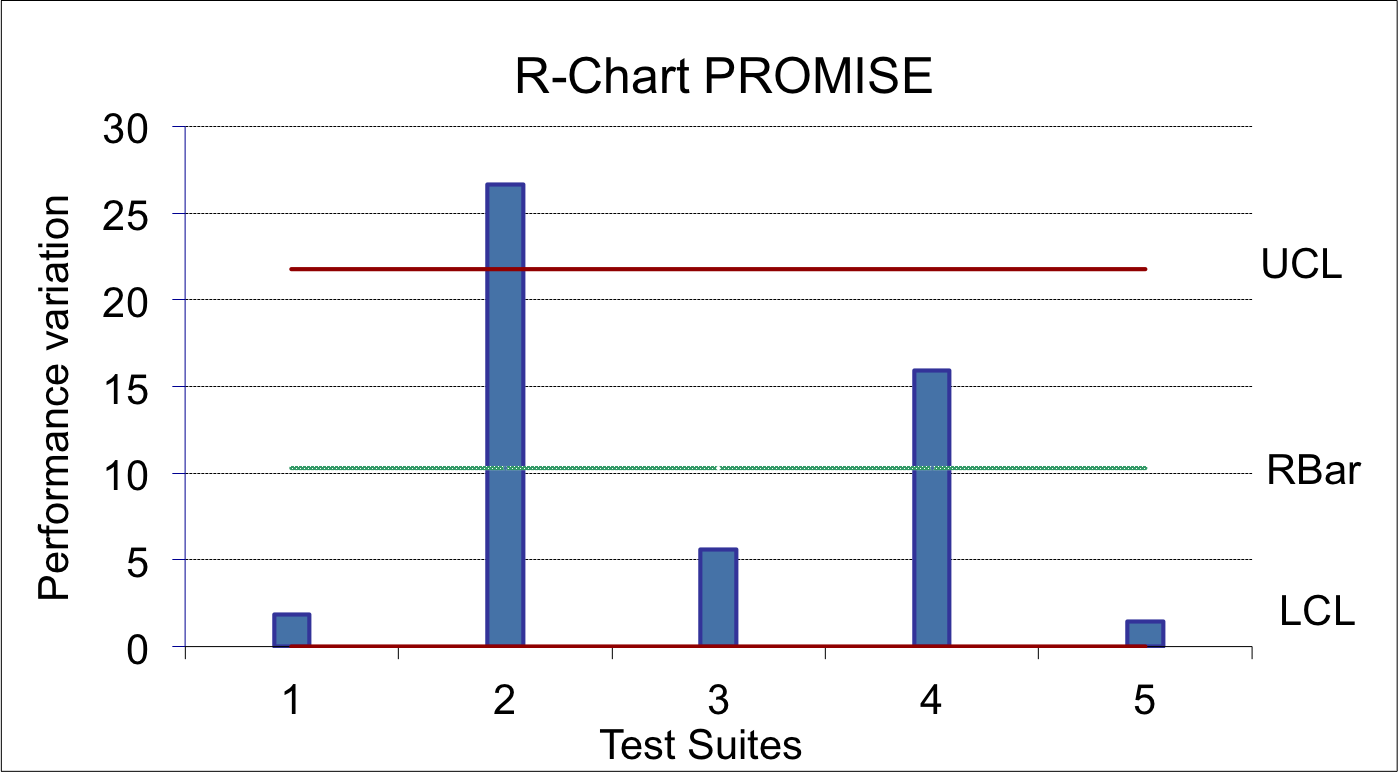
\includegraphics[width=0.48\linewidth]{chapitre4/fig/5.png}\label{rt5}}
	\subfigure[R-chart of the Culture benchmark program]{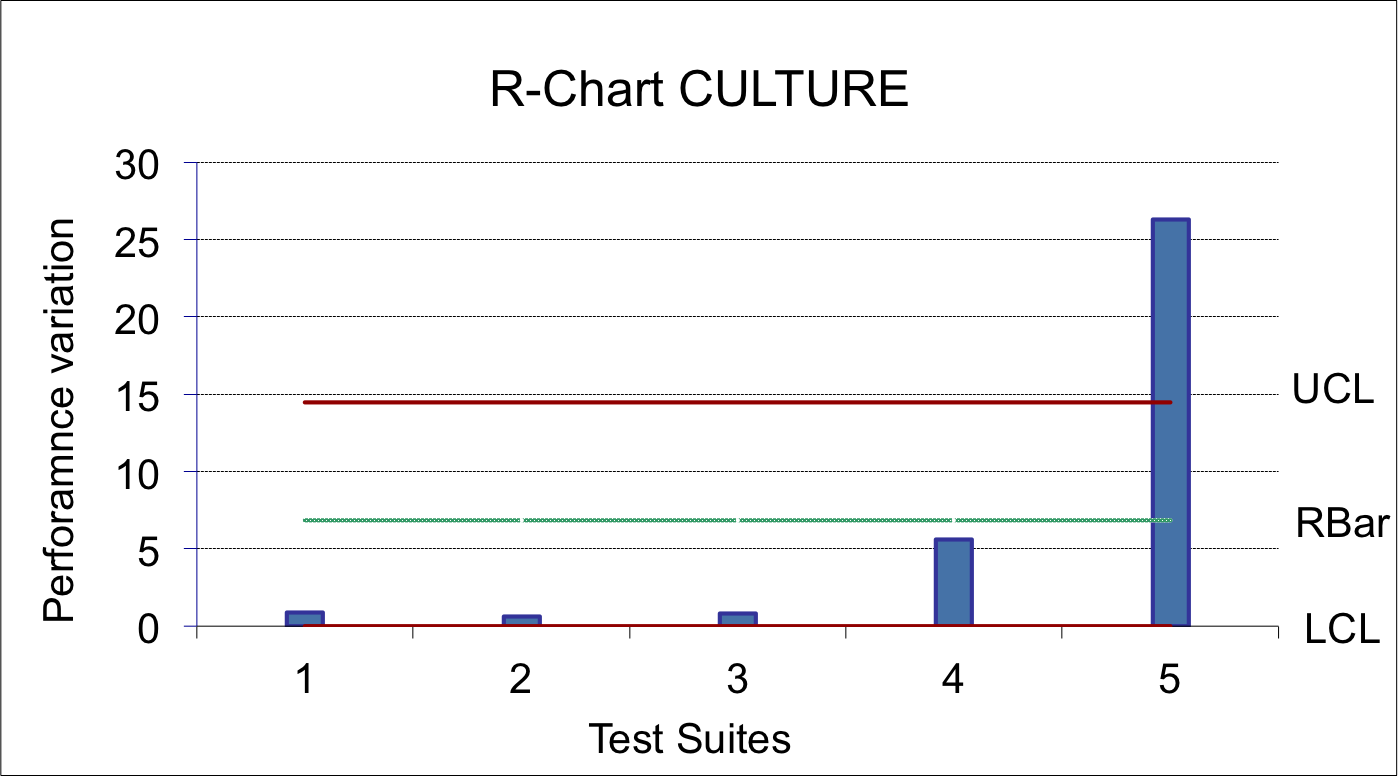
\includegraphics[width=0.48\linewidth]{chapitre4/fig/6.png}\label{rt6}}
	\subfigure[R-chart of the Math benchmark program]{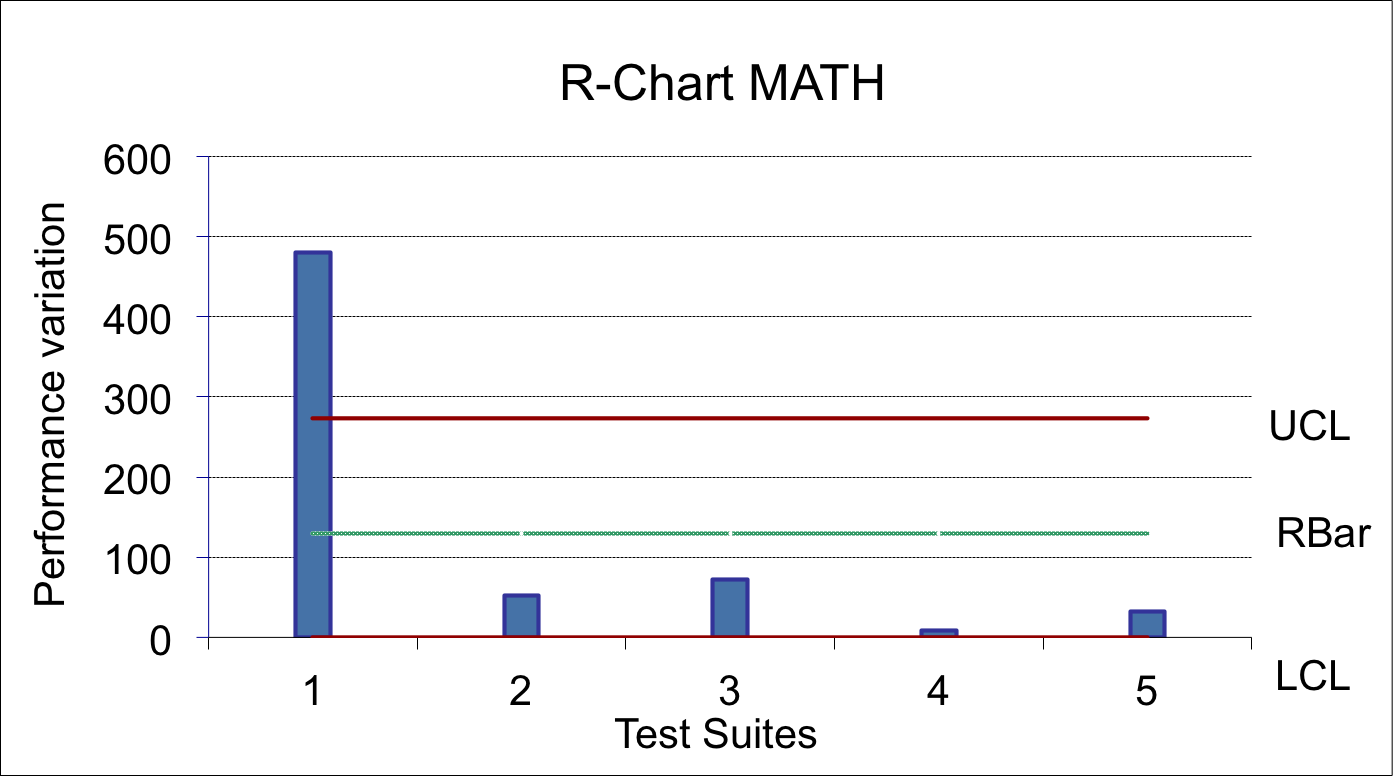
\includegraphics[width=0.48\linewidth]{chapitre4/fig/7.png}\label{rt7}}
	\caption{Performance variation of test suites across the different Haxe benchmarks}
	\label{rt}
\end{figure}

\begin{figure}
	\centering  
	\subfigure[R-chart of the Core benchmark program]{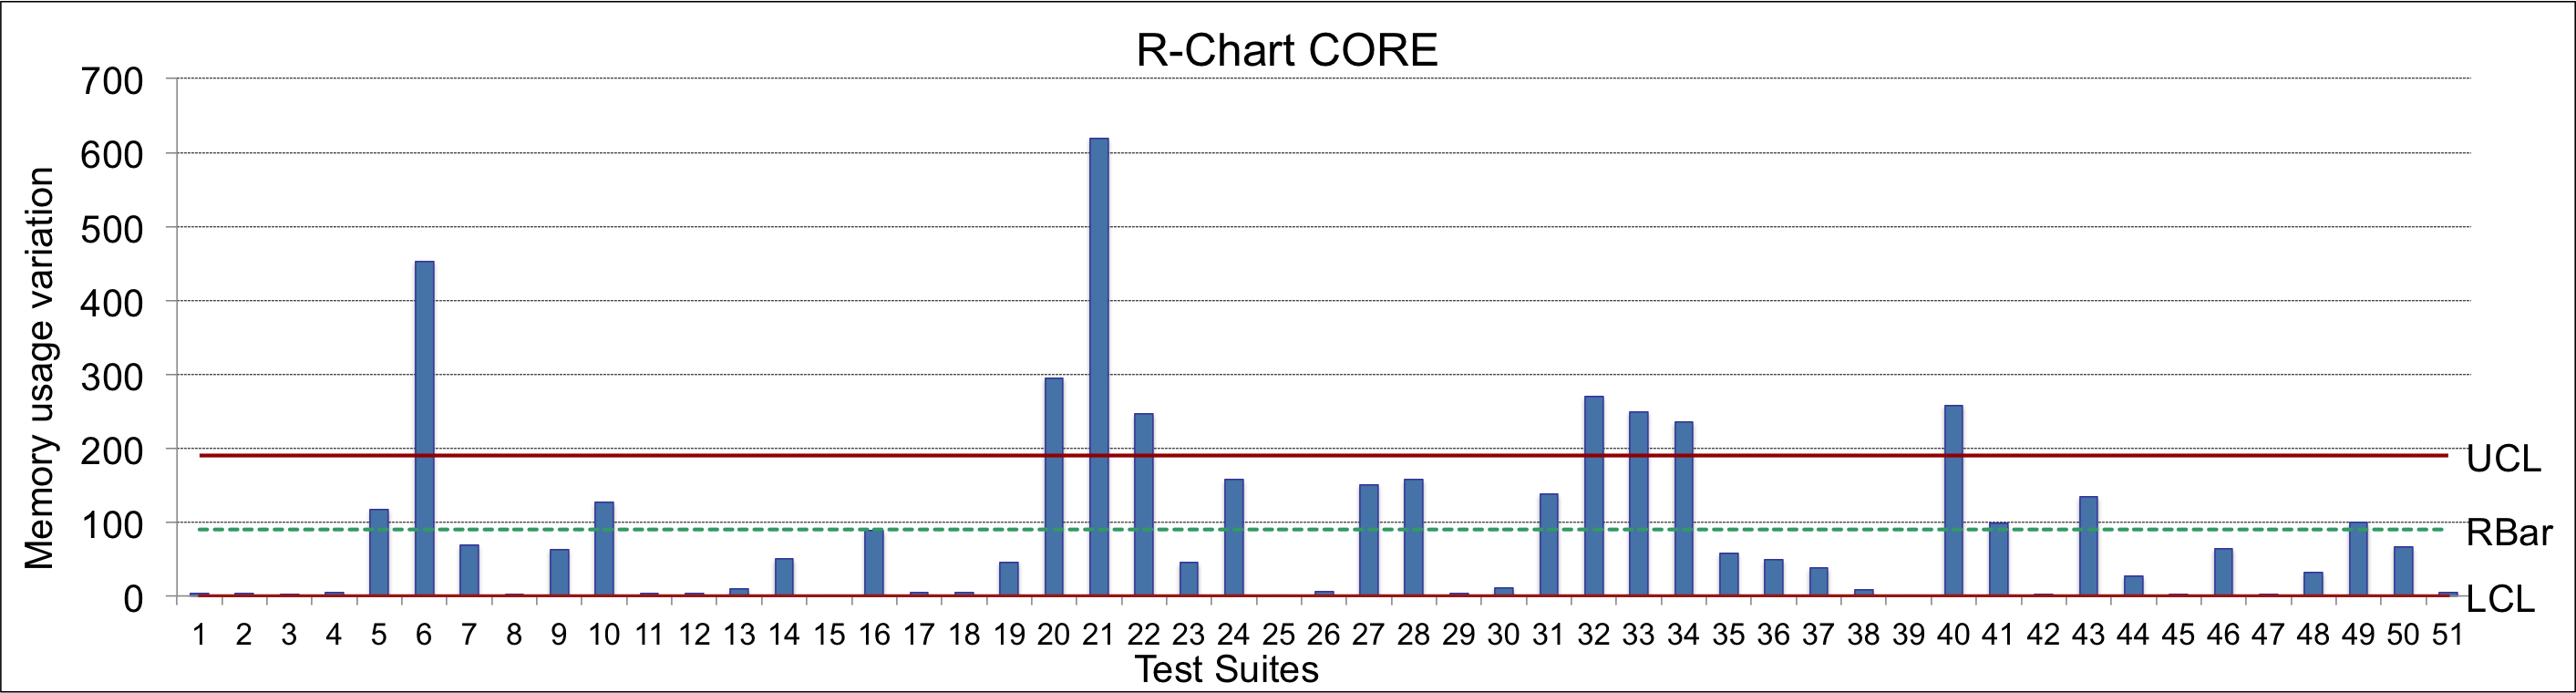
\includegraphics[width=0.96\linewidth]{chapitre4/fig/11.png}\label{rm1}}
	\subfigure[R-chart of the Color benchmark program]{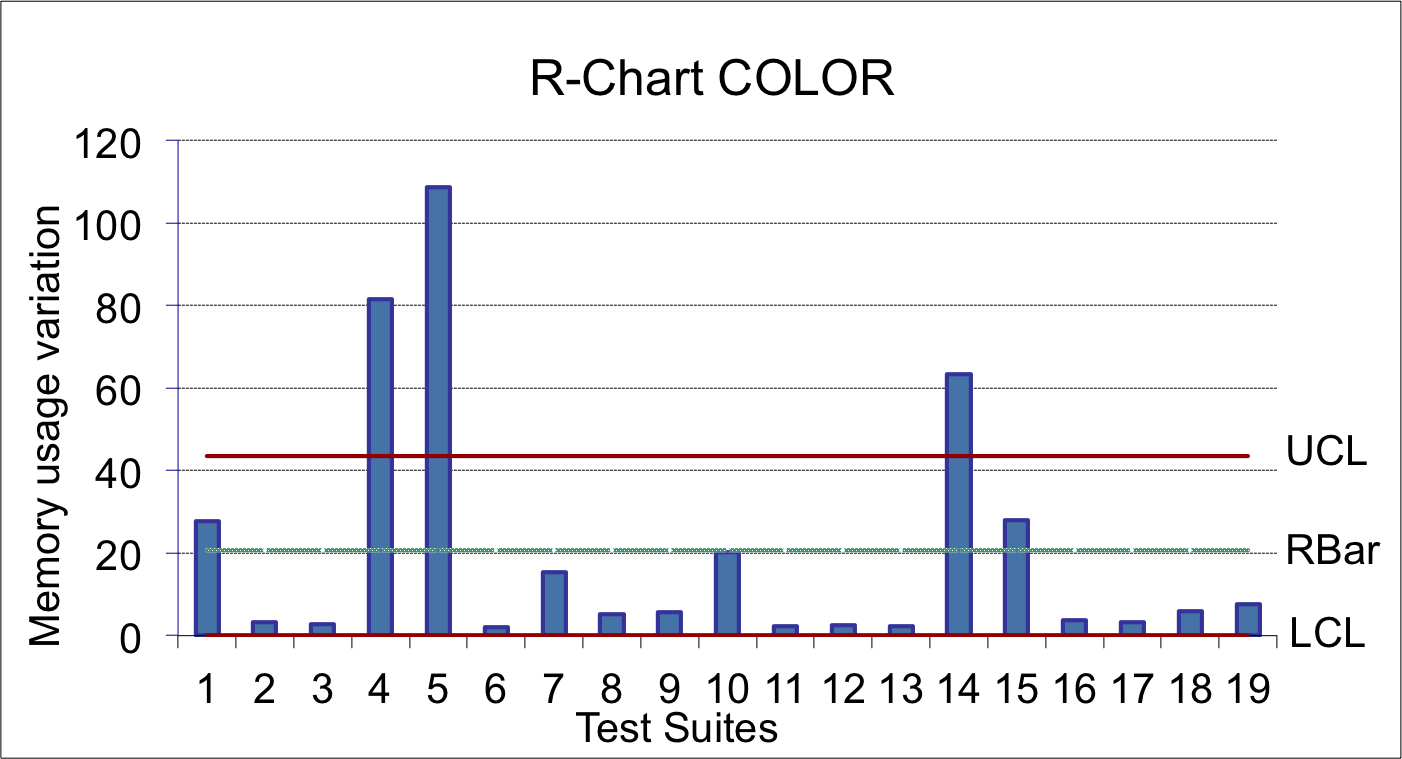
\includegraphics[width=0.48\linewidth]{chapitre4/fig/22.png}\label{rm2}}
	\subfigure[R-chart of the Hxmath benchmark program]{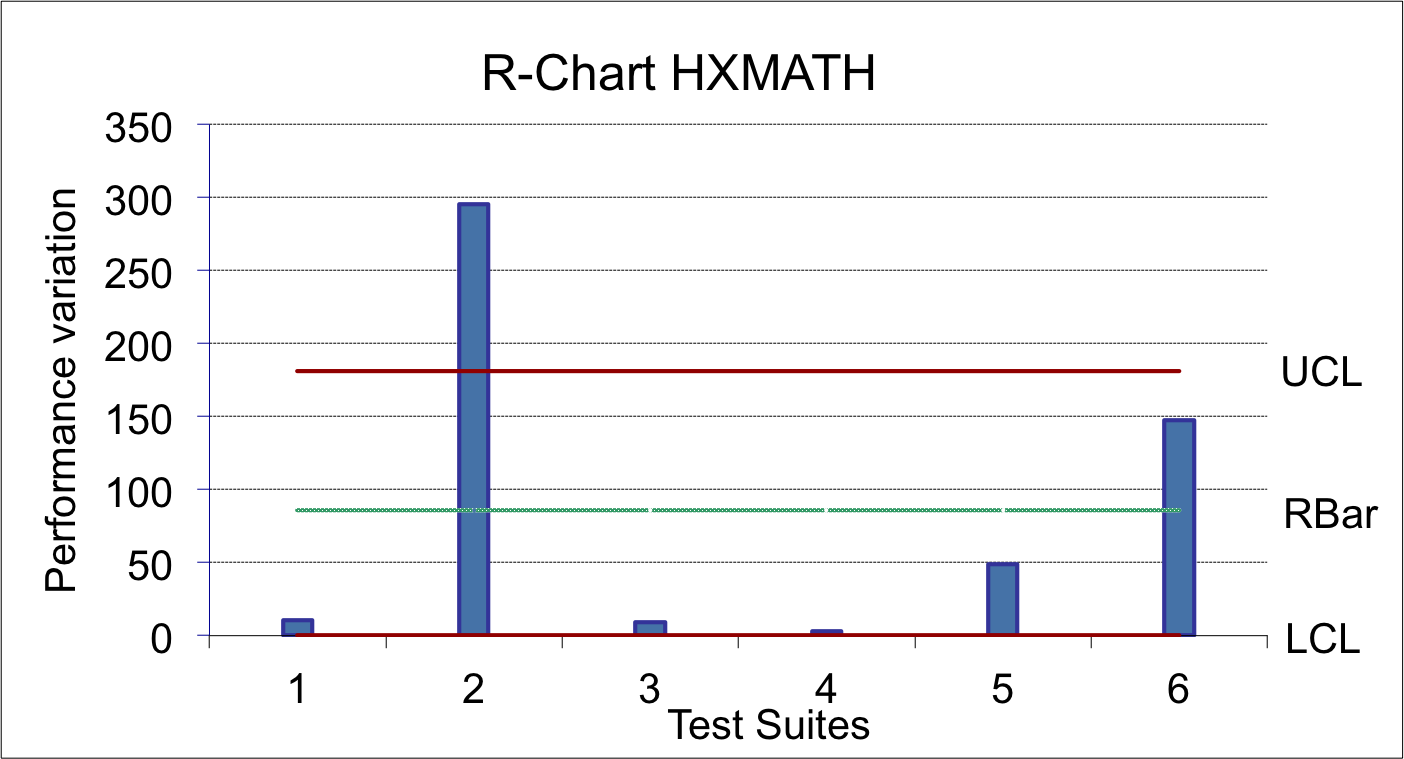
\includegraphics[width=0.48\linewidth]{chapitre4/fig/33.png}\label{rm3}}
	\subfigure[R-chart of the Format benchmark program]{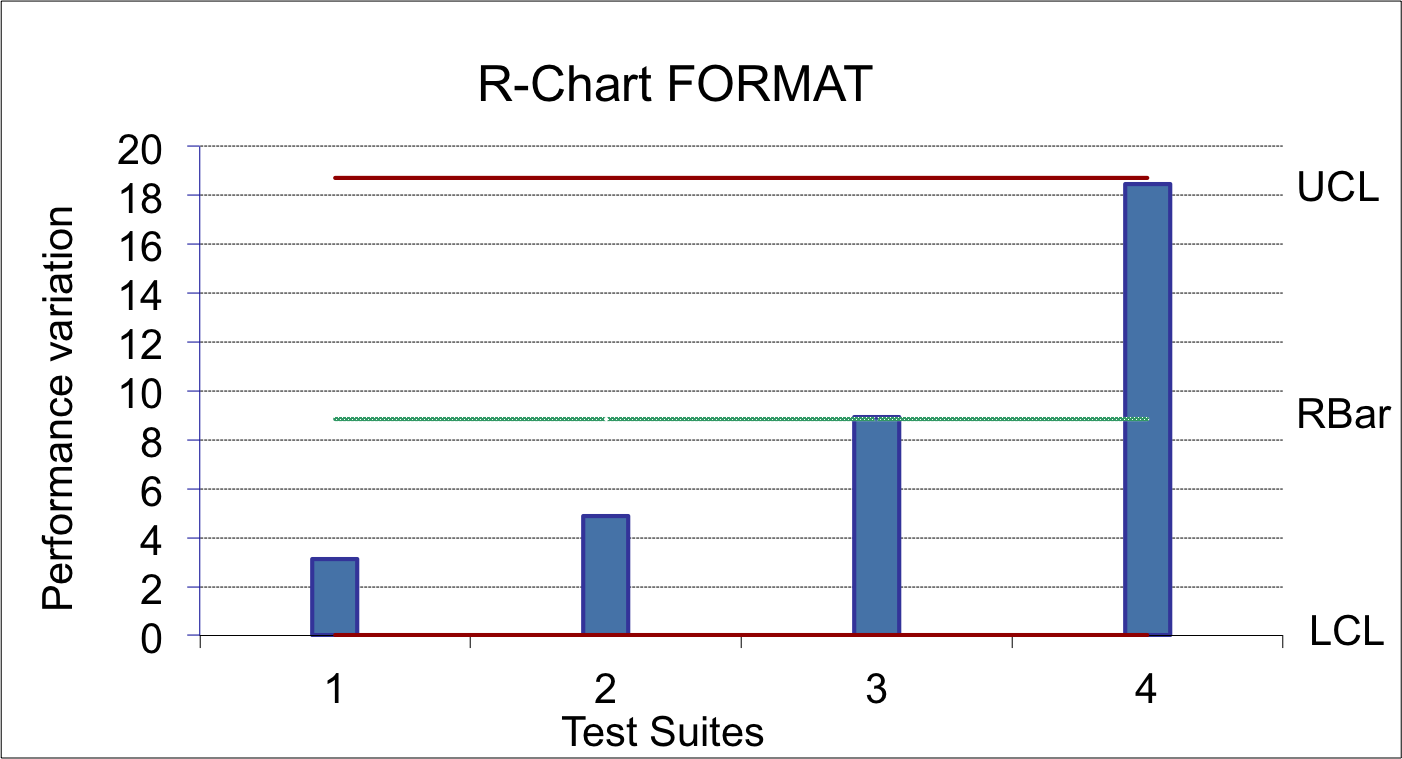
\includegraphics[width=0.48\linewidth]{chapitre4/fig/44.png}\label{rm4}}
	\subfigure[R-chart of the Promise benchmark program]{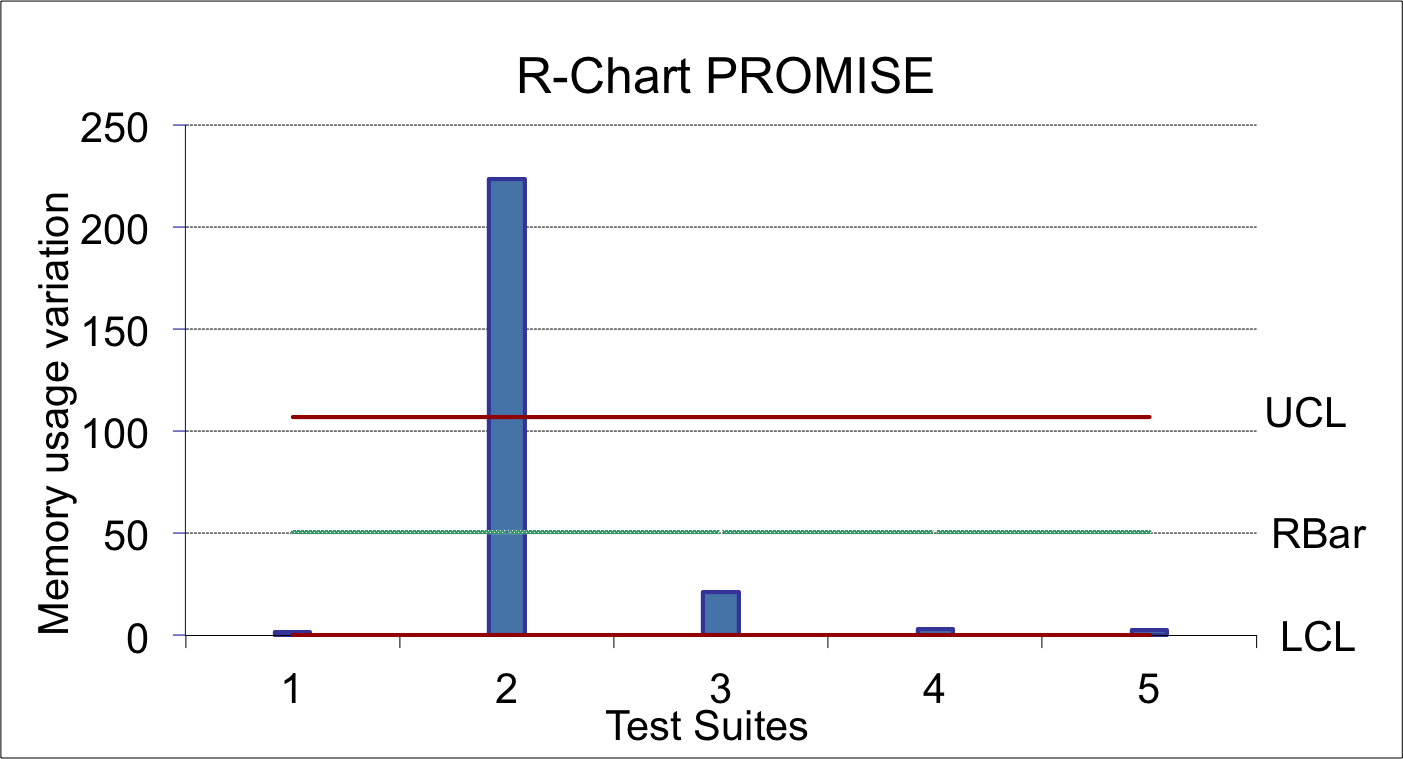
\includegraphics[width=0.48\linewidth]{chapitre4/fig/55.png}\label{rm5}}
	\subfigure[R-chart of the Culture benchmark program]{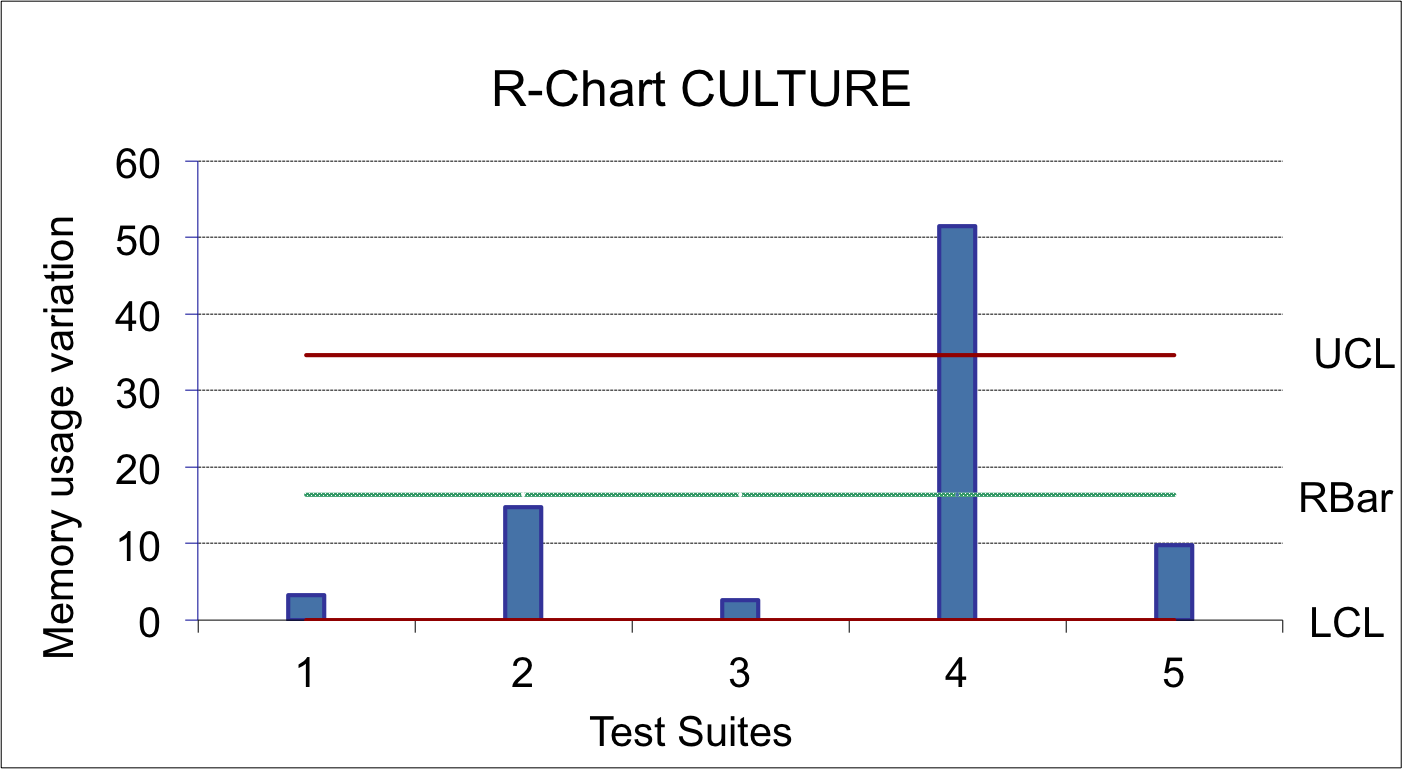
\includegraphics[width=0.48\linewidth]{chapitre4/fig/66.png}\label{rm6}}
	\subfigure[R-chart of the Math benchmark program]{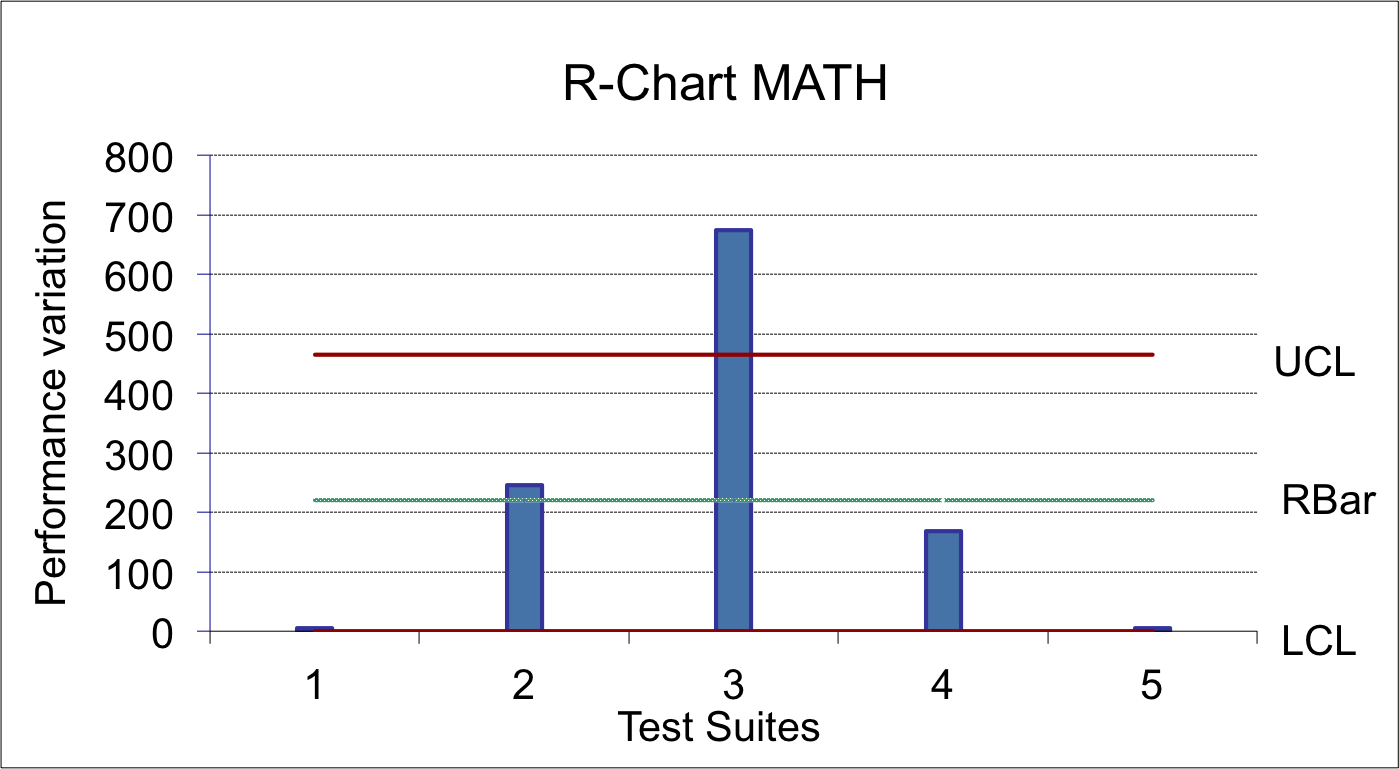
\includegraphics[width=0.48\linewidth]{chapitre4/fig/77.png}\label{rm7}}
	\caption{Memory usage variation of test suites across the different Haxe benchmarks}
	\label{rm}
\end{figure}
The results of R-charts for the seven benchmark programs relative to the performance and resource usage variation are reported in Figures \ref{rt} and \ref{rm}. For Figure \ref{rt}, we report the performance variation for each test suite corresponding to the range difference $R$ between the maximum and minimum execution time among the five targets (JAVA, JS, C++, C\#, and PHP). 
The execution time is of course scaled by dividing all values by the minimum execution time per test suite. 
The LCL for our experiments is always equal to 0 because the $D_{3}$ constant value as defined in equation \ref{eqUCL}, is equal to zero according to the R-chart constants table\footnote{\url{http://www.bessegato.com.br/UFJF/resources/table_of_control_chart_constants_old.pdf}}. In fact, the $D_{3}$ constant changes depending on the number of subgroups. In our experiments, our data record is composed of five subgroups corresponding to the five target programming languages.
The central line (in green) corresponds to $R$-$bar$. This value changes from one benchmark to another depending on the average of $R$ across all test suites in the benchmark. As a consequence, $UCL$, which is a function of $R$-$bar$, changes as long as we add new test suites to the experiments. $UCL$ is equal to $D_{4}*\bar{R}$ where $D_{4}=2.114$ according to the R-chart constants table. We recall that we have classified the R-chart approach as input sensitive since the average variation $R$-$bar$ and the threshold value $UCL$ change dynamically by adding new follow-up test suites to the corresponding benchmark. 
We note as well that these parameter values are appropriate to each benchmark program. We made this separation because we believe that the variation is highly dependent on the domain context and on the program under test. For example, testing the memory usage or performance of a program that performs a high mathematical computation (e.g., image processing, statistical analysis, etc) is not the same as a generated web application, since data types are handled differently. The R-charts used for measuring the memory usage variation follow the same concept as we have just been describing for performance variation.  

Results in Figure \ref{rt}, show that most of the performance variations are in the interval $[0-UCL]$, which corresponds to \textit{in-control} variation zone as it is described in Section \ref{sec:cg-Variation threshold}. However, we remark for several test suites that the performance variation becomes relatively high (higher than the $UCL$ value of the corresponding benchmark program). We detect 11 performance deviations lying in the \textit{out of control} variation zone. For the other test suites, the variation is even less than the total average variations $R$-$bar$. There are only 7 test suites among the remaining 84 ones where the variation lies in the interval $[\bar{R}-UCL]$. This variation is high but we are not detecting it asa performance deviation because according to the R-chart, variation in this zone is still \textit{in-control}. 
The 11 performance deviation we have detected can be explained by the fact that the execution time of one or more test suites varies considerably from one language to another. This argues the idea that the code generator has produced a suspect code behavior for one or more target language, which led to a high performance variation. We provide later better explanation in order to detect the faulty code generators.

Similarly, Figure \ref{rm} resumes the comparison results of test suites execution regarding the memory usage. The variation in this experiment are more important than previous results. This can be argued by the fact that the memory utilization and allocation patterns are different for each language. Nevertheless, we can recognize some points where the variation is extremely high. Thus, we detect 15 among 95 test suites that exceed the corresponding $UCL$ value. 
When the variation is below UCL, we detect 14 among the 80 remaining test suites where the variation lies in the interval $[\bar{R}-UCL]$, which is relatively high. 
One of the reasons that caused this variation may occur when the test suite executes some parts of the code (in a specific language) that are so greedy in terms of resources. This may not be the case when the variation is lower than the $\bar{R}$ for example.


To resume, we have detected 11 extreme performance variations and 15 extreme memory usage variations. We assume then, that faulty code generators, in identified points, represent a threat for software quality since the generated code has shown symptoms of poor-quality design. 



\paragraph{PCA results}~\\
\begin{figure}
	\centering  
	\subfigure[Test suites relative to the execution times ]{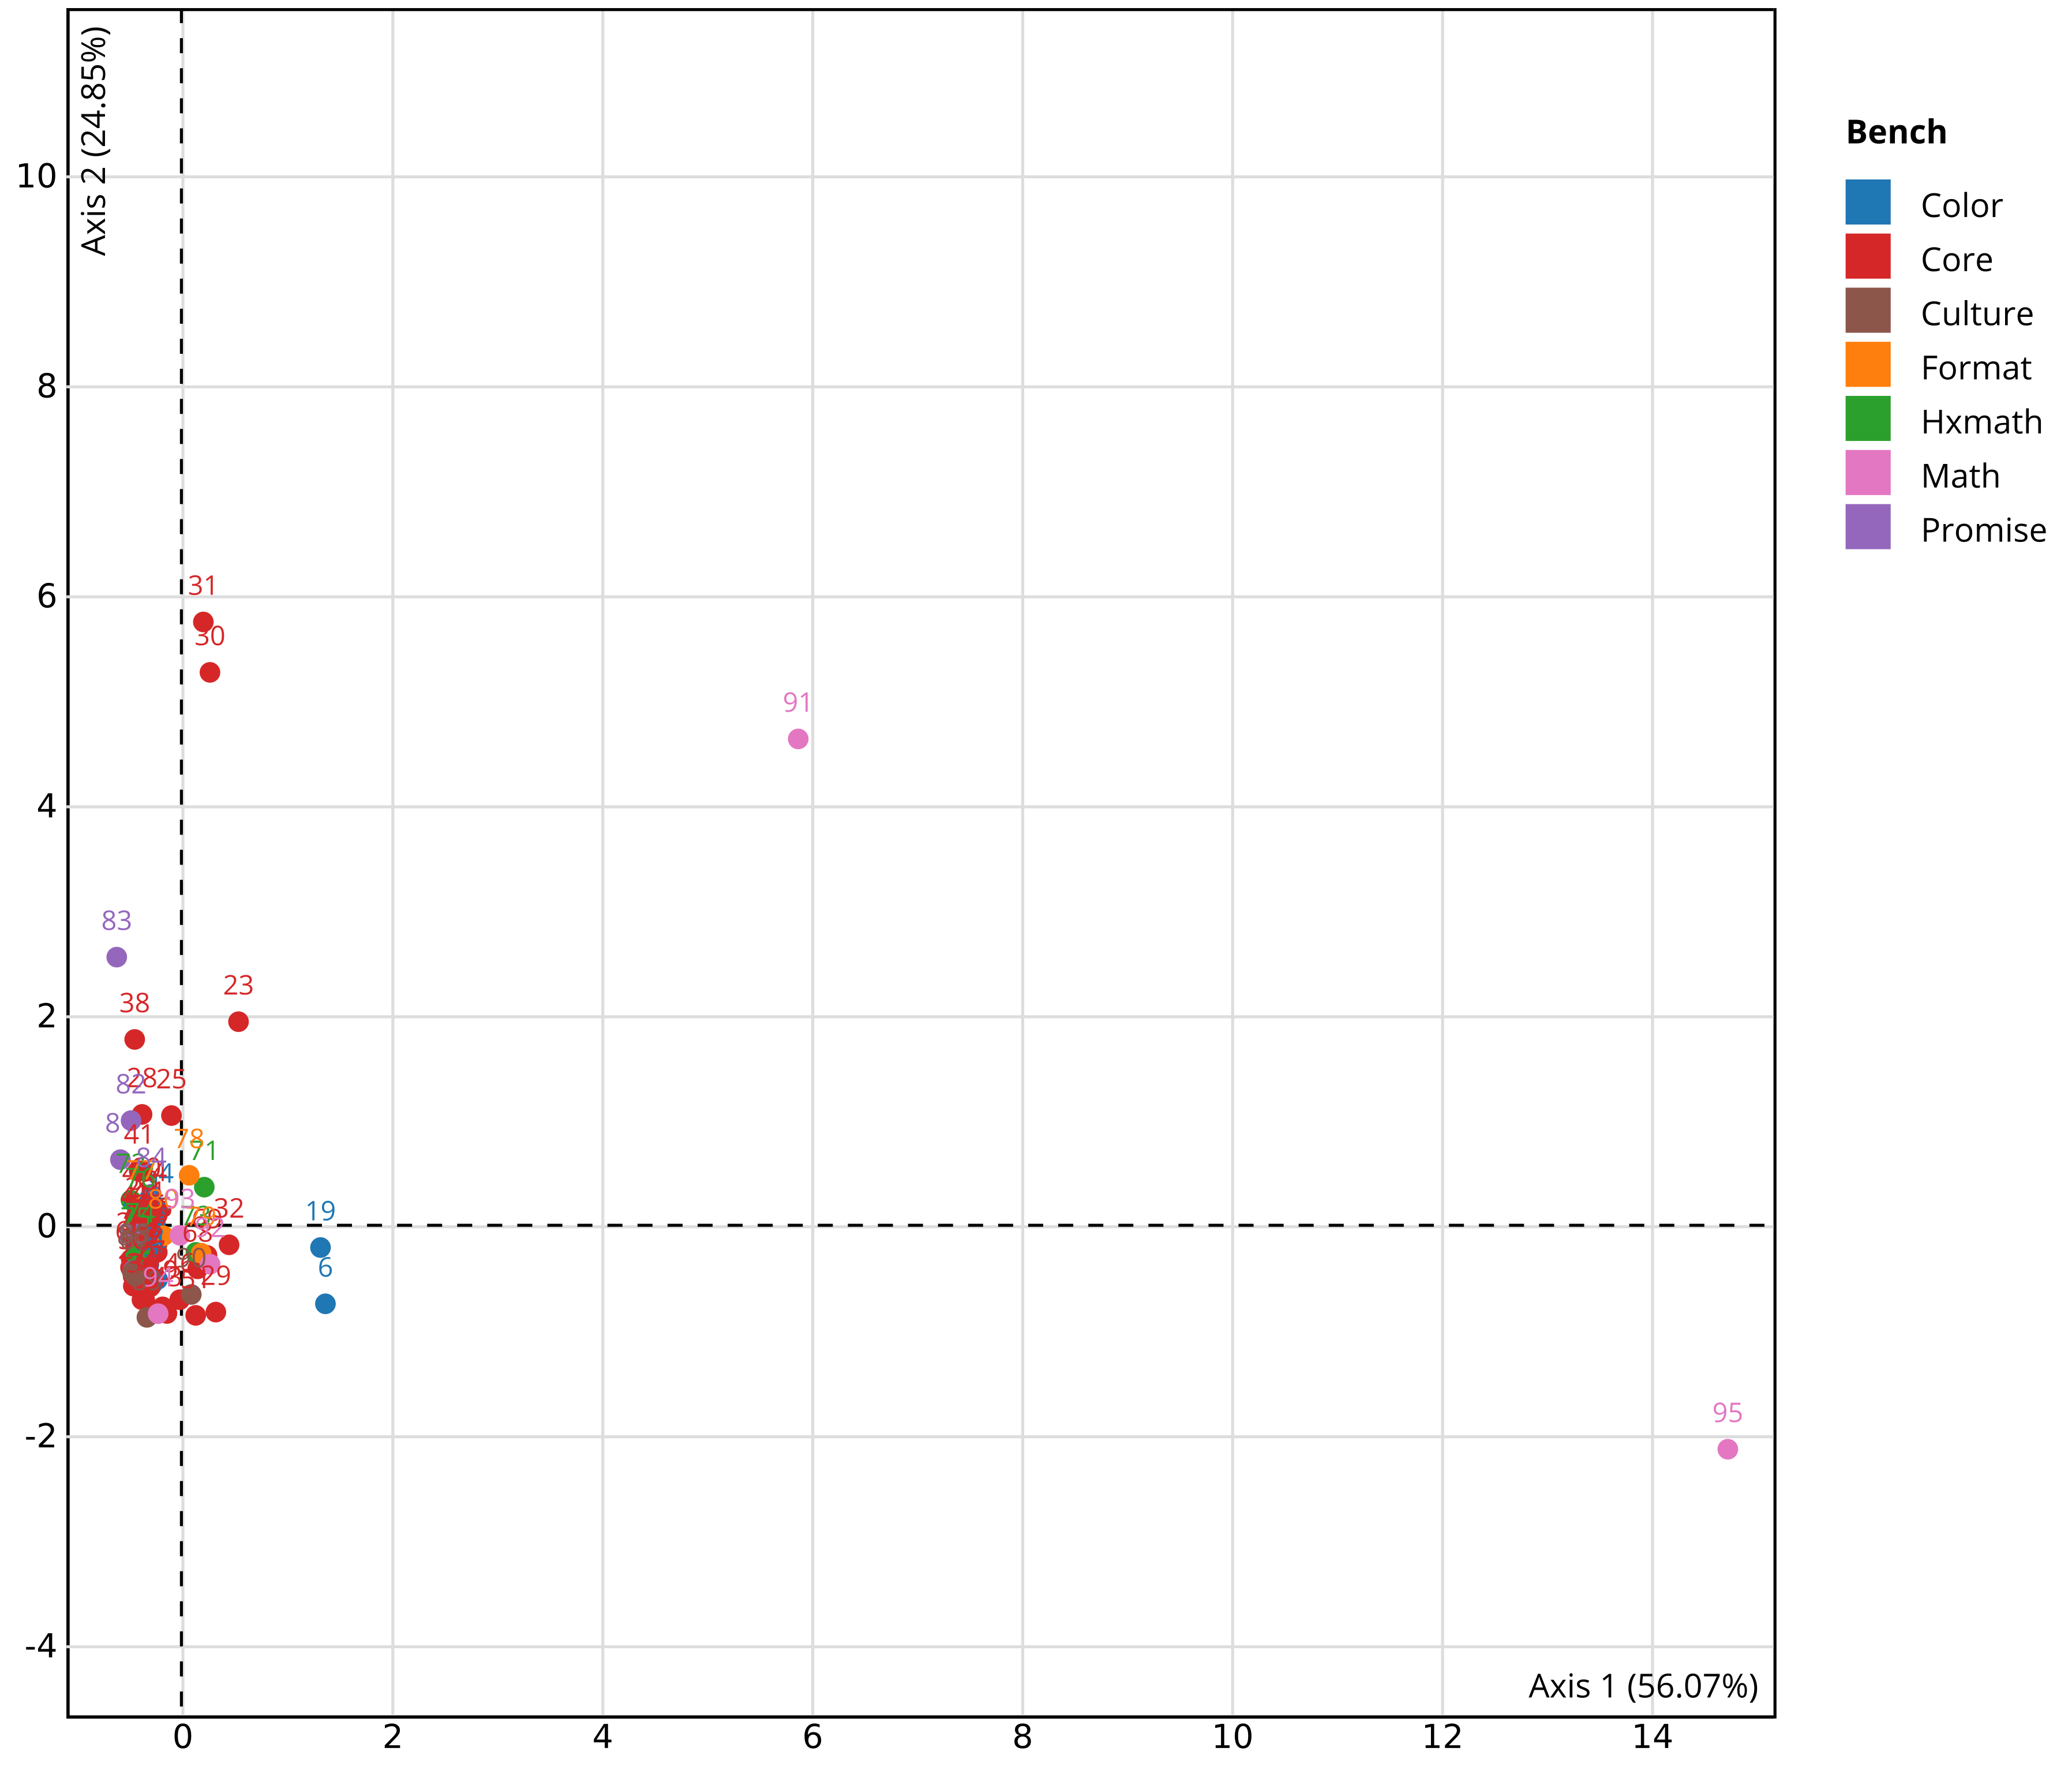
\includegraphics[width=0.7\linewidth]{chapitre4/fig/explor_ind}\label{pcat}}
	\subfigure[Test suites relative to the memory consumptions]{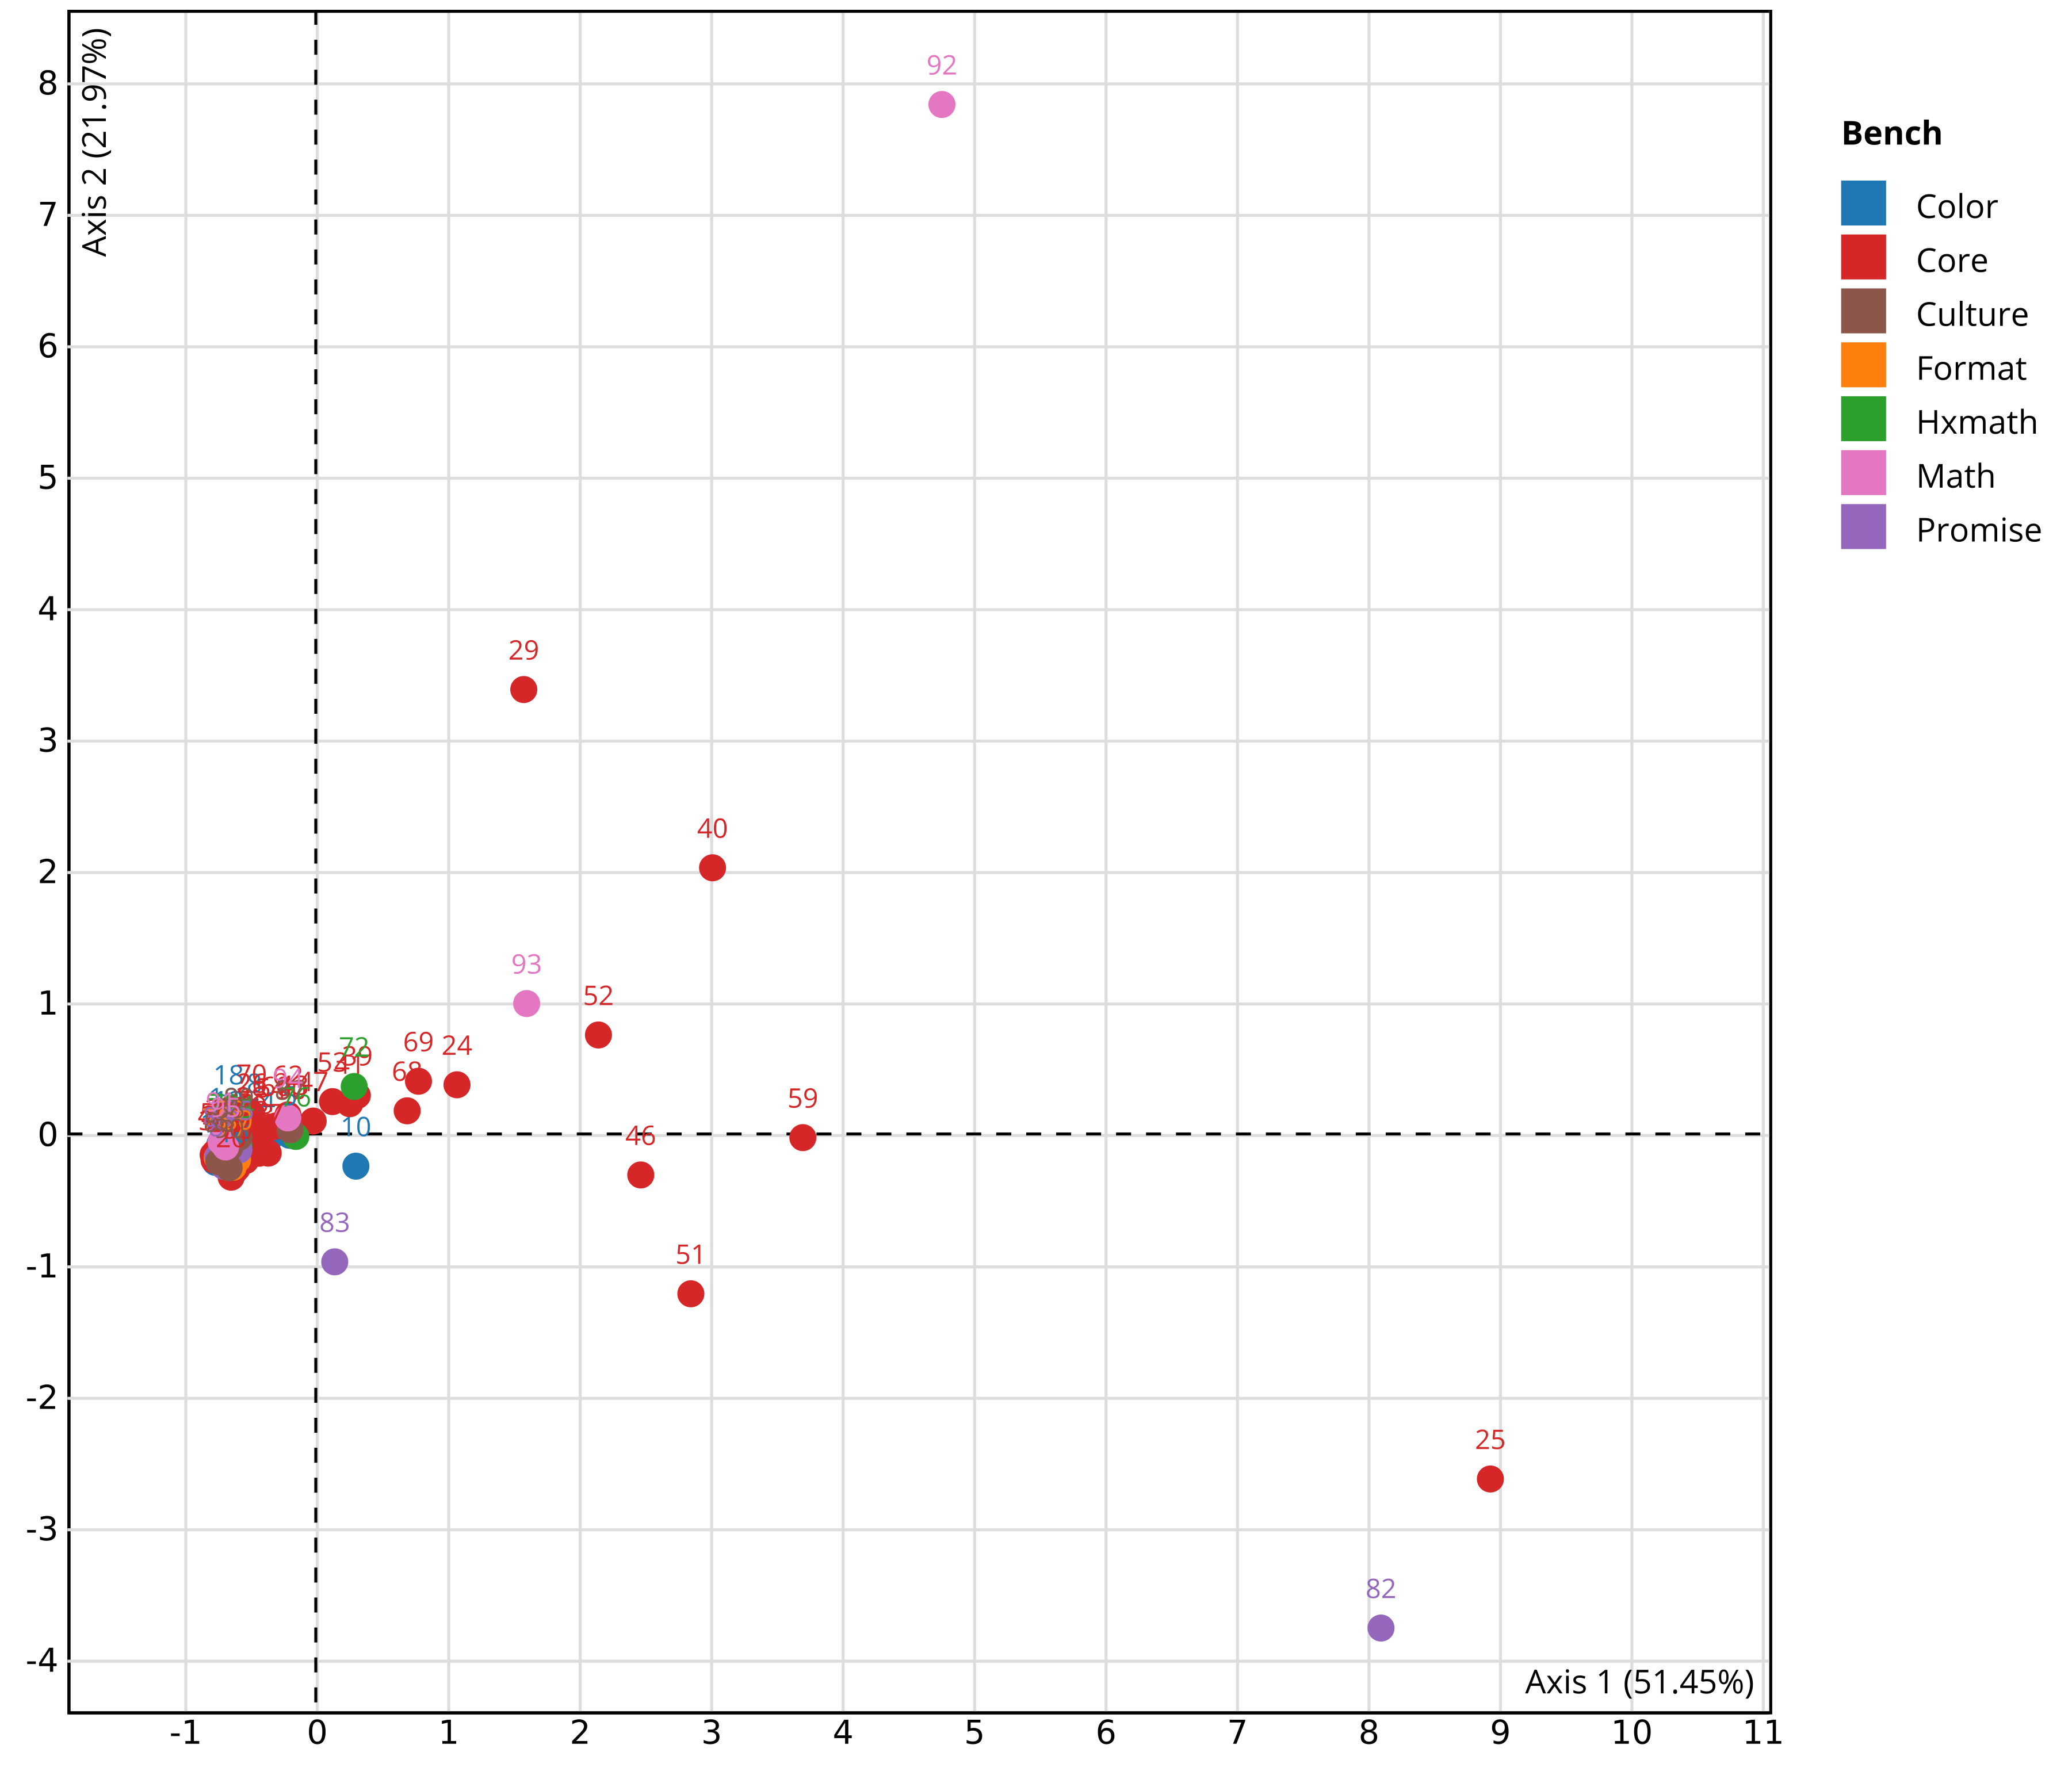
\includegraphics[width=0.7\linewidth]{chapitre4/fig/explor_ind2}\label{pcam}}
	\caption{PCAs showing the dispersion of our data over the PC subspace}
	\label{pca}
\end{figure}
\begin{figure}
	\centering  
	\subfigure[Performance deviations]{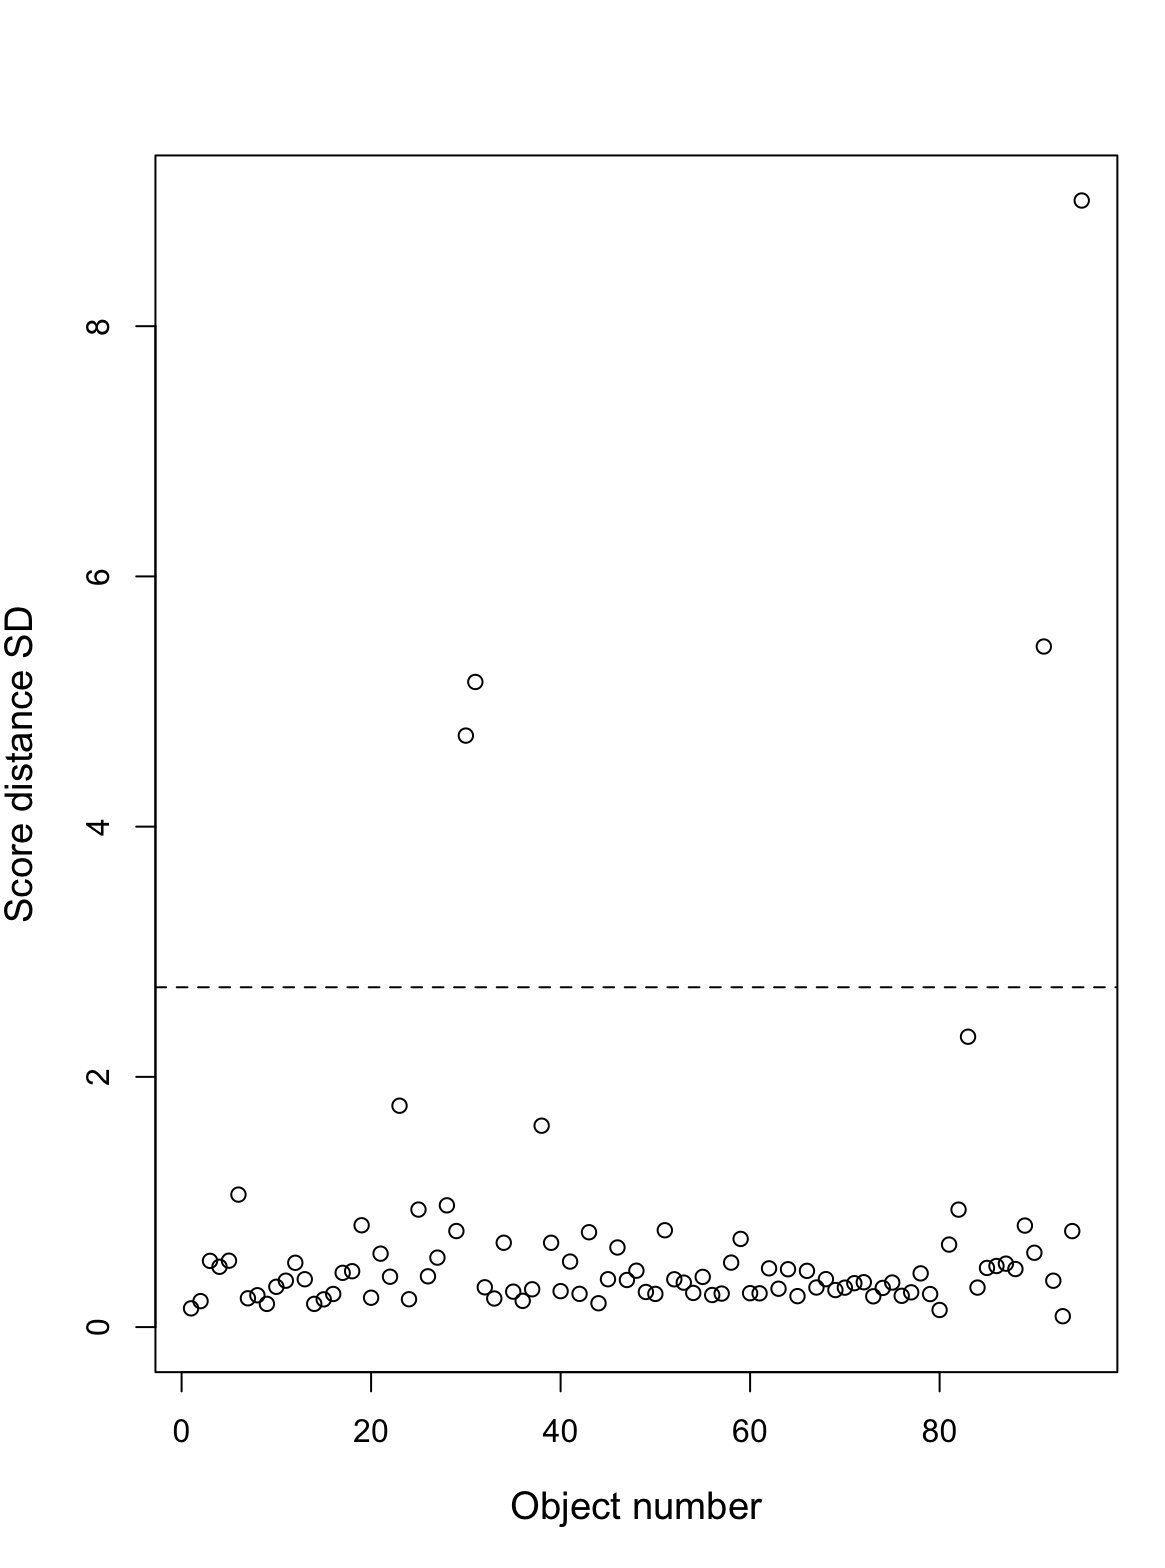
\includegraphics[width=0.49\linewidth]{chapitre4/fig/mahatime}\label{sdt}}
	\subfigure[Memory usage deviations]{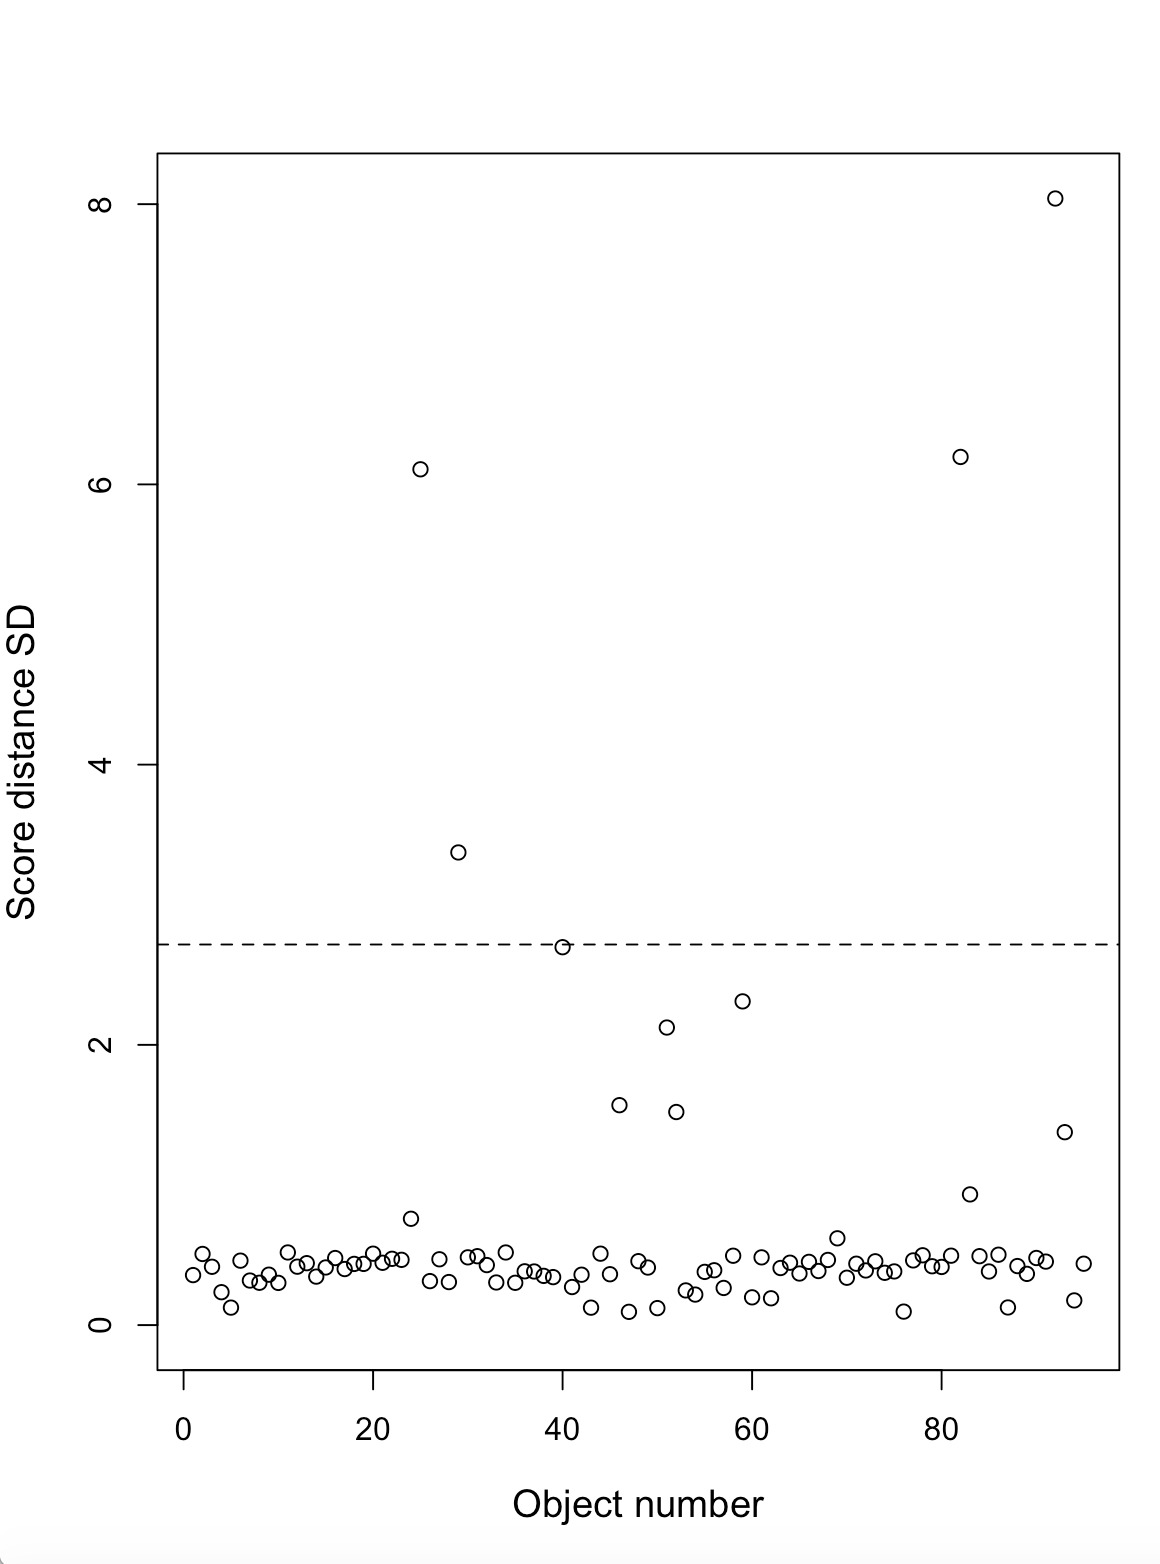
\includegraphics[width=0.49\linewidth]{chapitre4/fig/mahamem}\label{sdm}}
	
	\caption{Diagnostic plots using score distance SD. The vertical lines indicate critical values separating regular observations from outliers (97.5\%)}
	\label{sd}
\end{figure}
We apply the PCA approach as an alternative to the R-chart approach. Figure \ref{pca} shows the dispersion of our data points in the PC subspace. PC1 et PC2 represent the directions of our two first principal components, having the highest orthogonal variations. Our data points represent the performance variation (Figure \ref{pcat}) and the memory usage variation (Figure \ref{pcam}) of the 95 test suites we have executed. Variation points are colored according to benchmark program they belong to (displayed in the figure legend). At the first glance, we can clearly see that the variation points are situated in the same area except some points that lie far from this point cloud. In Figure \ref{pcat}, the pink points corresponding to the Math benchmark show visually the largest deviation from the point cloud. The three core test suites (in red) which are identified as performance deviations in R-chat, show also a deviation in the PCA scatter plot. Points 91 relative to the Math benchmark is deviating from the cloud point. However, in the R-chart diagram, it is not detected as a performance deviation (see the test suite 3 of Figure \ref{rt7}). In fact, this test suite takes more than 80 times to run. Compared to other test suites, the performance variation does not generally exceed 80. In effect, PCA performs a complete analysis of the whole data we have collected in all benchmarks. Thus, variations are displayed with respect to all test suites variations in all benchmarks. It is not limited to the variation inside the target benchmark program as we used to do using R-charts. We report the same results in Figure \ref{pcam} about the memory usage variation in the PCA. 


To confirm this observation, we present in Figure \ref{sd}, the results of applying our outliers detection approach to the previous presented PCAs. We identify 4 inconsistencies (or outliers) in each diagnostic plot. Inconsistencies in Figure \ref{pcat} are relative to the performance deviations. Points 31 and 32 correspond to the test suites 12 and 11 in benchmark Core of Figure \ref{rt1}. Points 91 and 95 correspond to the test suites 3 and 1 in benchmark Math of Figure \ref{rt7}. For memory usage variation, we detect points 25, 29, 82, and 92 which corresponds relatively to the test suites 21 and 6 of benchmark Core, 2 of benchmark Promise, and 3 of benchmark Math.
We can clearly see that this technique help to identify only the extreme value outliers. We used 97.5\%-Quantile to define the cutoff value that is commonly used in the literature\cite{enot2008preprocessing,hubert2009robust}. If we decrease this value we will be able to detect more variation points. 


\paragraph{Detected inconsistencies }~\\
\begin{table*}[h]
	\centering
	
	\resizebox{\columnwidth}{!}{%
		\begin{tabular}{|c|c|c|c|c|c|c|c|c|}
			\hline
			\textbf{Benchamrk}                & \textbf{Test Suite}            & \textbf{JAVA} & \textbf{JS} & \textbf{CPP} & \textbf{CS} & \textbf{PHP}                   & \textbf{UCL(R)}         & \textbf{Defective CG} \\ \hline
			\textbf{Color}                    & \textbf{TS19}                  & 1.90          & 1           & 2.37         & 3.31        & \cellcolor[HTML]{E3E3E3}61.84  & 13.08                   & PHP                   \\ \hline
			&                                & 1             & 1.59        & 1.67         & 2.78        & \cellcolor[HTML]{E3E3E3}148.20 &                         & PHP                   \\ \cline{3-7} \cline{9-9} 
			&                                & 1.14          & 2.71        & 1            & 3.63        & \cellcolor[HTML]{E3E3E3}258.94 &                         & PHP                   \\ \cline{3-7} \cline{9-9} 
			&                                & 1.28          & 2.94        & 1            & 3.36        & \cellcolor[HTML]{E3E3E3}261.36 &                         & PHP                   \\ \cline{3-7} \cline{9-9} 
			\multirow{-4}{*}{\textbf{Core}}   & \multirow{-4}{*}{\textbf{TS4}} & 1             & 1.05        & 1.86         & 2.39        & \cellcolor[HTML]{E3E3E3}50.30  & \multirow{-4}{*}{43.62} & PHP                   \\ \hline
			&                                & 2.38          & 1.43        & 1            & 2.82        & \cellcolor[HTML]{E3E3E3}51.72  &                         & PHP                   \\ \cline{3-7} \cline{9-9} 
			\multirow{-2}{*}{\textbf{Hxmath}} & \multirow{-2}{*}{\textbf{TS1}} & 2.14          & 1.10        & 1            & 2.25        & \cellcolor[HTML]{E3E3E3}50.56  & \multirow{-2}{*}{42.97} & PHP                   \\ \hline
			\textbf{Format}                   & \textbf{TS2}                   & 1.16          & 1.27        & 1            & 3.35        & \cellcolor[HTML]{E3E3E3}81.85  & 70.66                   & PHP                   \\ \hline
			\textbf{Promise}                  & \textbf{TS2}                   & 1.52          & 1.85        & 1            & 1.51        & \cellcolor[HTML]{E3E3E3}27.67  & 21.76                   & PHP                   \\ \hline
			\textbf{Culture}                  & \textbf{TS5}                   & 1.62          & 1           & 1.27         & 2.02        & \cellcolor[HTML]{E3E3E3}27.29  & 14.47                   & PHP                   \\ \hline
			\textbf{Math}                     & \textbf{TS1}                   & 4.15          & 1           & 5.41         & 4.70        & \cellcolor[HTML]{E3E3E3}481.68 & 273.24                  & PHP                   \\ \hline
		\end{tabular}%
	}
	\caption{Raw data values of test suites that led to the highest variation in terms of execution time}
	\label{perf-tab}`
\end{table*}

\begin{table*}[h]
	\centering
	
	\resizebox{\columnwidth}{!}{%
		\begin{tabular}{|c|c|c|c|c|c|c|c|c|}
			\hline
			\textbf{Benchmark}               & \textbf{Test suite} & \textbf{JAVA}                  & \textbf{JS} & \textbf{CPP} & \textbf{CS} & \cellcolor[HTML]{FFFFFF}\textbf{PHP} & \textbf{UCL}             & \textbf{Defective CG} \\ \hline
			& \textbf{TS4}        & 1                              & 2.29        & 1.47         & 3.59        & \cellcolor[HTML]{E8E8E8}82.46        &                          & PHP                   \\ \cline{2-7} \cline{9-9} 
			& \textbf{TS5}        & 1                              & 3.08        & 1.83         & 4.53        & \cellcolor[HTML]{E8E8E8}109.69       &                          & PHP                   \\ \cline{2-7} \cline{9-9} 
			\multirow{-3}{*}{\textbf{Color}} & \textbf{TS14}       & 1                              & 1.32        & 1.00         & 2.03        & \cellcolor[HTML]{E8E8E8}64.45        & \multirow{-3}{*}{43.53}  & PHP                   \\ \hline
			& \textbf{TS6}        & \cellcolor[HTML]{E8E8E8}250.77 & 71.71       & 1            & 69.90       & \cellcolor[HTML]{E8E8E8}454.15       &                          & PHP \& JAVA           \\ \cline{2-7} \cline{9-9} 
			& \textbf{TS20}       & 2.31                           & 1.34        & 1            & 3.27        & \cellcolor[HTML]{E8E8E8}296.10       &                          & PHP                   \\ \cline{2-7} \cline{9-9} 
			& \textbf{TS21}       & 11.90                          & 1           & 14.63        & 36.18       & \cellcolor[HTML]{E8E8E8}620.22       &                          & PHP                   \\ \cline{2-7} \cline{9-9} 
			& \textbf{TS22}       & 1                              & 2.70        & 1.74         & 4.69        & \cellcolor[HTML]{E8E8E8}247.32       &                          & PHP                   \\ \cline{2-7} \cline{9-9} 
			& \textbf{TS32}       & \cellcolor[HTML]{E8E8E8}270.78 & 2.27        & 1            & 5.61        & 153.37                               &                          & JAVA                  \\ \cline{2-7} \cline{9-9} 
			& \textbf{TS33}       & 1.82                           & 1.12        & 1            & 54.19       & \cellcolor[HTML]{E8E8E8}250.35       &                          & PHP                   \\ \cline{2-7} \cline{9-9} 
			& \textbf{TS34}       & 1                              & 1.17        & 1.48         & 3.90        & \cellcolor[HTML]{E8E8E8}236.97       &                          & PHP                   \\ \cline{2-7} \cline{9-9} 
			\multirow{-8}{*}{\textbf{Core}}  & \textbf{TS40}       & 160.84                         & 1.10        & 1            & 49.43       & \cellcolor[HTML]{E8E8E8}259.20       & \multirow{-8}{*}{190.03} & PHP                   \\ \hline
			\textbf{Hxmath}                  & \textbf{TS2}        & 1                              & 1.16        & 1.91         & 2.82        & \cellcolor[HTML]{E8E8E8}296.16       & 181.11                   & PHP                   \\ \hline
			\textbf{Promise}                 & \textbf{TS2}        & \cellcolor[HTML]{E8E8E8}214.53 & 92.45       & 1            & 57.68       & \cellcolor[HTML]{E8E8E8}224.41       & 106.82                   & PHP \& JAVA           \\ \hline
			\textbf{Culture}                 & \textbf{TS4}        & 2.75                           & 1.01        & 2.52         & 1           & \cellcolor[HTML]{E8E8E8}52.47        & 34.63                    & PHP                   \\ \hline
			\textbf{Math}                    & \textbf{TS3}        & 1.29                           & 1           & 1.72         & 3.60        & \cellcolor[HTML]{E8E8E8}675.00       & 464.80                   & PHP                   \\ \hline
		\end{tabular}%
	}
	\caption{Raw data values of test suites that led to the highest variation in terms of memory usage}
	\label{mem-tab}`
\end{table*}

Now that we have observed the performance and memory usage variations of test suites execution, we can analyze the extreme points we have detected using R-chart to observe in greater depth the source of such deviation.
For that reason, we present in Table \ref{perf-tab} and \ref{mem-tab} the raw data values of these test suites leading to an extreme variation in terms of execution time and memory usage. We report the inconsistencies gathered from the first approach, R-chart.

Table \ref{perf-tab} shows the execution time factor of each test suite execution in a specific target language. This factor is scaled with respect to the the lowest execution time among the five targets. We also report the $UCL$ defined per benchmark. In the last column, we report the code generator that caused such large deviation. To do so, we designate by defective CG the code generator in where the test suite execution time factor exceeds the $UCL$ value.

We can clearly see that the PHP code has a singular behavior regarding the performance with a factor ranging from x27.29 for test suite 5 in benchmark Culture (Format\_TS3) to x481.7 for Math\_TS1. For example, if Math\_TS1 takes $1$ minute to run in JS, the same test suite in PHP will take around $8$ hours to run which is a very large gap. 
The highest factor detected for other languages is x5.41 which is not negligible but it represents a small deviation compared to PHP deviations. While it is true that we are comparing different versions of generated code, it was expected to get some variations while running test cases in terms of execution time. However, in the case of PHP code generator, it is far to be a simple variation but it is more likely to be a code generator inconsistency that led to such performance regression.


Meanwhile, we gathered information about the points that led to the highest variation in terms of memory usage. Table \ref{mem-tab} shows these results. 
Again, we can identify a singular behavior of the PHP code regarding the memory usage with a factor ranging from x52.47 to x675. For other test suites versions, the factor varies from x1 to x160.84. We observe as well a singular behavior of the JAVA code for Core\_TS6, Core\_TS32, and Promise\_TS2 yielding to a variation higher than the $UCL$. 
These results prove that the PHP and JAVA code generators are not always effective and they constitute a threat for the generated software in terms of memory usage.

%Besides the performance issues of PHP code generator presented in table~5, the results of memory usage confirm our claim since the PHP code has the highest memory utilization.

The inconsistencies we found are more related to the incorrect memory utilization patterns produced by the defective code generator, or by generating a non-optimized and efficient code . Such inconsistencies may come from an inadequate type usage, high resource instantiation, etc.
To give more insights about the source of this issue, we provide in the following further analysis of these inconsistencies.



\subsubsection{Analysis}


%Our testing infrastructure allows to automatically detect inconsistencies among a set of code generators. 
These inconsistencies need to be fixed by code generator creators in order to enhance the code quality of generated code (PHP code for example). Since we are proposing a black-box testing approach, our solution is not able to provide more precise and detailed information about the part of code that has caused these performance issue, which is one of the limitations of our testing approach.

Thus, to understand this particular singular performance of the PHP code when applying the test suite Core\_TS4 for example, we looked (manually) into the PHP code corresponding to this test suite. In fact, we observe the intensive use of \textit{"arrays"} in most of the functions under test. Arrays are known to be slow in PHP and PHP library has introduced much more advanced functions such as $array\_fill$ and specialized abstract types such as \textit{"SplFixedArray"}\footnote{\url{http://php.net/manual/fr/class.splfixedarray.php}} to overcome this limitation. So, by changing just these two parts in the generated code, we improve the PHP code speed with a factor x5 which is very valuable. We also reduce the memory usage of this test suite by a factor of x2.

In short, the lack of use of specific types, in native PHP standard library, by the PHP code generator such as \textit{SplFixedArray} shows a real impact on the non-functional behavior of generated code. In contrast, selecting carefully the adequate types and functions to generate code can lead to performance improvement. The types used in the code generator are not the best ones. 

\subsection{Threats to validity}
We resume, in the following paragraphs, external and internal threats that can be raised:

\textit{External validity} refers to the generalizability of our findings. In this study, we perform experiments on Haxe and on a set of test suite selected from Github and from the Haxe community. For instance, we have no guarantee that these libraries cover all the Haxe language features neither than all the Haxe standard libraries. Consequently, we cannot guarantee that our approach is able to find all the code generators issues unless we develop a more comprehensive test suite. Moreover, the threshold defined to detect the singular performance behavior has a huge impact on the precision and recall of the proposed approach. Experiments should be replicated to other case studies to confirm our findings and try to understand the best heuristic to detect the code generator issues regarding performance (i.e., automatically calculate the threshold values)

\textit{Internal validity} is concerned with the use of a container-based approach. Even if it exists emulators such as Qemu\footnote{\url{https://goo.gl/SxKG1e}} that allow to reflect the behavior of heterogeneous hardware, the chosen infrastructure has not been evaluated to test generated code that target heterogeneous hardware machines. In addition, even though system containers are known to be lightweight and less resource-intensive compared to full-stack virtualization, we would validate the reliability of our approach by comparing it with a non-virtualized approach in order to see the impact of using containers on the accuracy of the results.



%hrough these conducted experiments, we reached interesting results, some of which were unexpected.


%In most languages, arrays are fixed-sized, but this is not the case in PHP since they are allocated dynamically. The dynamic allocation of arrays  leads to a slower write time because the memory locations needed to hold the new data is not already allocated. Thus, slow writing speed damages the performance of PHP code and impact the memory usage. This observation clearly confirm our early findings. The solution for this problem may be to use another type of object from the Standard PHP Library. As an alternative, \textit{"SplFixedArray"} pre-allocates the necessary memory and allows a faster array implementation, thereby solving the issue of slower write times. [ref to spl benchs]

%\subsection{Discussions}
%For instance, the poor performance of the Haxe-produced PHP code was certainly a surprise. 
%The PHP target had a very large execution time and memory usage for almost every test suite execution. 
%That is to say that PHP code generator is clearly generating non-efficient code regarding the non-functional properties. It is even possible to say that other code generators are not extremely efficient since we found that C++ code consumed, during one test suite execution (Color\_TS6), more memory than PHP. But, we cannot say for sure that C++ code generator is buggy. Thus, we cannot make any assumption. Nevertheless, the only point which, at this stage, can be statistically made is that PHP code generator has a real performance issue that has to be fixed by code generators developers. 

%In attempting to understand the reasons of this PHP performance issues, we tried to take a look at the source code generated in PHP. As an example, we looked at the source code of Core\_TS4. 




\section{Conclusion}
\label{sec:cg-conclusion}
Our approach is a black-box testing technique and it does not provide detailed information about the source of the issues. Nevertheless, we rather provide a mechanism to detect these potential issues within a set of code generator families so that, these issues may be investigated and fixed afterwards by code generators/software maintainers. 



In this work we have described a new approach for testing and monitoring the code generators families using a container-based infrastructure. 
We used a set of micro-services in order to provide a fine-grained understanding of resource consumption. 
To validate our approach, we evaluate a popular family of code generators: HAXE. 
The evaluation results show that we can find real issues in existing code generators. 
In particular, we show that we could find two kinds of errors: the lack of use of a specific function and an abstract type that exist in the standard library of the target language which can reduce the memory usage/execution time of the resulting program.

As a current work, we are discussing with the Haxe community to submit a patch with the first findings. 
We are also conducting the same evaluation for two other code generators families: ThingML and TypeScript. 
As a future work, we are going to improve our understanding on the threshold which can provide a best precision for detecting performance issues in code generators. 
In this paper, we detected inconsistencies related to the execution speed and memory usage. In the future, we seek, using the same testing infrastructure, to detect more code generator inconsistencies related to other non-functional metrics such CPU consumption, etc. 






\iffalse
\begin{table}[h]
	\centering	
	\resizebox{\columnwidth}{!}{%
		\begin{tabular}{|l|l|S[table-format=3.2]|l|S[table-format=3.2]|l|S[table-format=3.2]|}
			\hline
			\textbf{Benchmark}                 & \textbf{TestSuite} & \textbf{Std\_dev}                & \textbf{TestSuite} & \textbf{Std\_dev}             & \textbf{TestSuite} & \textbf{Std\_dev}              \\ \hline
			& \textbf{TS1}       & 0.55                             & \textbf{TS8}       & 0.24                          & \textbf{TS15}      & 0.73                           \\ \cline{2-7} 
			& \textbf{TS2}       & 0.29                             & \textbf{TS9}       & 0.22                          & \textbf{TS16}      & 0.12                           \\ \cline{2-7} 
			& \textbf{TS3}       & 0.34                             & \textbf{TS10}      & 0.10                          & \textbf{TS17}      & 0.31                           \\ \cline{2-7} 
			& \textbf{TS4}       & 2.51                             & \textbf{TS11}      & 0.17                          & \textbf{TS18}      & 0.34                           \\ \cline{2-7} 
			& \textbf{TS5}       & 1.53                             & \textbf{TS12}      & 0.28                          & \textbf{TS19}      & \cellcolor[HTML]{C0C0C0}120.61 \\ \cline{2-7} 
			& \textbf{TS6}       & 43.50                            & \textbf{TS13}      & 0.33                         & \multicolumn{2}{l|}{\multirow{2}{*}{}} \\ \cline{2-5}
			\multirow{-7}{*}{\textbf{Color}}   & \textbf{TS7}       & 0.50                             & \textbf{TS14}      & 1.88                          & \multicolumn{2}{l|}{}                  \\ \hline
			& \textbf{TS1}       & 0.35                             & \textbf{TS18}      & 0.16                          & \textbf{TS35}      & 1.30                           \\ \cline{2-7} 
			& \textbf{TS2}       & 0.07                             & \textbf{TS19}      & 0.60                          & \textbf{TS36}      & 1.13                           \\ \cline{2-7} 
			& \textbf{TS3}       & 0.30                             & \textbf{TS20}      & 5.79                          & \textbf{TS37}      & 2.02                           \\ \cline{2-7} 
			& \textbf{TS4}       & \cellcolor[HTML]{C0C0C0}27299.89 & \textbf{TS21}      & 0.47                          & \textbf{TS38}      & 0.26                           \\ \cline{2-7} 
			& \textbf{TS5}       & 6.12                             & \textbf{TS22}      & 2.74                          & \textbf{TS39}      & 0.16                           \\ \cline{2-7} 
			& \textbf{TS6}       & 21.90                            & \textbf{TS23}      & 2.14                          & \textbf{TS40}      & 8.12                           \\ \cline{2-7} 
			& \textbf{TS7}       & 0.41                             & \textbf{TS24}      & 3.79                          & \textbf{TS41}      & 5.45                           \\ \cline{2-7} 
			& \textbf{TS8}       & 0.28                             & \textbf{TS25}      & 0.19                          & \textbf{TS42}      & 0.11                           \\ \cline{2-7} 
			& \textbf{TS9}       & 0.78                             & \textbf{TS26}      & 0.13                          & \textbf{TS43}      & 1.41                           \\ \cline{2-7} 
			& \textbf{TS10}      & 1.82                             & \textbf{TS27}      & 5.59                          & \textbf{TS44}      & 1.56                           \\ \cline{2-7} 
			& \textbf{TS11}      & \cellcolor[HTML]{C0C0C0}180.68   & \textbf{TS28}      & 1.71                          & \textbf{TS45}      & 0.11                           \\ \cline{2-7} 
			& \textbf{TS12}      & \cellcolor[HTML]{C0C0C0}185.02   & \textbf{TS29}      & 0.26                          & \textbf{TS46}      & 1.04                           \\ \cline{2-7} 
			& \textbf{TS13}      & \cellcolor[HTML]{C0C0C0}128.78   & \textbf{TS30}      & 0.44                          & \textbf{TS47}      & 0.23                           \\ \cline{2-7} 
			& \textbf{TS14}      & 0.71                             & \textbf{TS31}      & 1.71                          & \textbf{TS48}      & 1.34                           \\ \cline{2-7} 
			& \textbf{TS15}      & 0.12                             & \textbf{TS32}      & 2.42                          & \textbf{TS49}      & 1.86                           \\ \cline{2-7} 
			& \textbf{TS16}      & 0.65                             & \textbf{TS33}      & 8.29                          & \textbf{TS50}      & 1.28                           \\ \cline{2-7} 
			\multirow{-17}{*}{\textbf{Core}}   & \textbf{TS17}      & 0.26                             & \textbf{TS34}      & 5.25                          & \textbf{TS51}      & 3.53                           \\ \hline
			& \textbf{TS1}       & 31.65                            & \textbf{TS3}       & 30.34                         & \textbf{TS5}       & 0.40                           \\ \cline{2-7} 
			\multirow{-2}{*}{\textbf{Hxmath}}  & \textbf{TS2}       & 4.27                             & \textbf{TS4}       & 0.25                          & \textbf{TS6}       & 0.87                           \\ \hline
			& \textbf{TS1}       & 0.28                             & \textbf{TS3}       & \cellcolor[HTML]{C0C0C0}95.36 & \textbf{TS4}       & 1.49                           \\ \cline{2-7} 
			\multirow{-2}{*}{\textbf{Format}}  & \textbf{TS2}       & \cellcolor[HTML]{C0C0C0}64.94    & \multicolumn{4}{l|}{\textbf{}}                                                                           \\ \hline
			\textbf{Promise}                   & \textbf{TS1}       & 0.29                             & \textbf{TS2}       & 13.21                         & \textbf{TS3}       & 1.21                           \\ \hline
			& \textbf{TS1}       & 0.13                             & \textbf{TS3}       & 0.13                          & \textbf{TS4}       & 1.40                           \\ \cline{2-7} 
			\multirow{-2}{*}{\textbf{Culture}} & \textbf{TS2}       & 0.10                             & \multicolumn{4}{l|}{}                                                                                    \\ \hline
			\textbf{Math}                      & \textbf{TS1}       & \cellcolor[HTML]{C0C0C0}642.85   & \textbf{TS2}       & 28.32                         & \textbf{TS3}       & 24.40                          \\ \hline
		\end{tabular}%
	}
	
	\caption{The comparison results of running each test suite across five target languages: the metric used is the standard deviation between execution times  }
	\label{tab:The comparison results1}
\end{table}

% Please add the following required packages to your document preamble:
% \usepackage{multirow}
% Please add the following required packages to your document preamble:
% \usepackage{multirow}
% \usepackage[table,xcdraw]{xcolor}
% If you use beamer only pass "xcolor=table" option, i.e. \documentclass[xcolor=table]{beamer}
\begin{table}[]
	\centering
	
	\resizebox{\columnwidth}{!}{%
		\begin{tabular}{|l|l|S[table-format=3.2]|l|S[table-format=3.2]|l|S[table-format=3.2]|}
			\hline
			\textbf{Benchmark}                 & \textbf{TestSuite} & \textbf{Std\_dev}               & \textbf{TestSuite} & \textbf{Std\_dev}              & \textbf{TestSuite} & \textbf{Std\_dev}              \\ \hline
			& \textbf{TS1}       & 10.19                           & \textbf{TS8}       & 1.23                           & \textbf{TS15}      & 14.44                          \\ \cline{2-7} 
			& \textbf{TS2}       & 1.17                            & \textbf{TS9}       & 1.95                           & \textbf{TS16}      & 1.13                           \\ \cline{2-7} 
			& \textbf{TS3}       & 0.89                            & \textbf{TS10}      & 1.27                           & \textbf{TS17}      & 0.72                           \\ \cline{2-7} 
			& \textbf{TS4}       & 30.34                           & \textbf{TS11}      & 0.57                           & \textbf{TS18}      & 0.97                           \\ \cline{2-7} 
			& \textbf{TS5}       & 31.79                           & \textbf{TS12}      & 1.11                           & \textbf{TS19}      & \cellcolor[HTML]{C0C0C0}777.32 \\ \cline{2-7} 
			& \textbf{TS6}       & \cellcolor[HTML]{C0C0C0}593.05  & \textbf{TS13}      & 0.46                           & \multicolumn{2}{l|}{}                               \\ \cline{2-5}
			\multirow{-7}{*}{\textbf{Color}}   & \textbf{TS7}       & 12.14                           & \textbf{TS14}      & 45.90                          & \multicolumn{2}{l|}{\multirow{-2}{*}{}}             \\ \hline
			& \textbf{TS1}       & 1.40                            & \textbf{TS18}      & 1.00                           & \textbf{TS35}      & 14.13                          \\ \cline{2-7} 
			& \textbf{TS2}       & 1.17                            & \textbf{TS19}      & 20.37                          & \textbf{TS36}      & 32.41                          \\ \cline{2-7} 
			& \textbf{TS3}       & 0.60                            & \textbf{TS20}      & 128.23                         & \textbf{TS37}      & 22.72                          \\ \cline{2-7} 
			& \textbf{TS4}       & \cellcolor[HTML]{C0C0C0}403.15  & \textbf{TS21}      & 24.38                          & \textbf{TS38}      & 2.19                           \\ \cline{2-7} 
			& \textbf{TS5}       & 41.95                           & \textbf{TS22}      & 76.24                          & \textbf{TS39}      & 0.26                           \\ \cline{2-7} 
			& \textbf{TS6}       & 203.55                          & \textbf{TS23}      & 18.82                          & \textbf{TS40}      & 126.29                         \\ \cline{2-7} 
			& \textbf{TS7}       & 19.69                           & \textbf{TS24}      & 72.01                          & \textbf{TS41}      & 31.01                          \\ \cline{2-7} 
			& \textbf{TS8}       & 0.78                            & \textbf{TS25}      & 0.21                           & \textbf{TS42}      & 0.93                           \\ \cline{2-7} 
			& \textbf{TS9}       & 30.41                           & \textbf{TS26}      & 2.30                           & \textbf{TS43}      & 50.36                          \\ \cline{2-7} 
			& \textbf{TS10}      & 57.19                           & \textbf{TS27}      & 101.53                         & \textbf{TS44}      & 12.56                          \\ \cline{2-7} 
			& \textbf{TS11}      & 68.92                           & \textbf{TS28}      & 43.67                          & \textbf{TS45}      & 0.91                           \\ \cline{2-7} 
			& \textbf{TS12}      & 74.19                           & TS29               & 0.90                           & \textbf{TS46}      & 27.28                          \\ \cline{2-7} 
			& \textbf{TS13}      & 263.99                          & \textbf{TS30}      & 4.02                           & \textbf{TS47}      & 1.10                           \\ \cline{2-7} 
			& \textbf{TS14}      & 19.89                           & \textbf{TS31}      & 52.35                          & \textbf{TS48}      & 15.40                          \\ \cline{2-7} 
			& \textbf{TS15}      & 0.30                            & \textbf{TS32}      & 134.75                         & \textbf{TS49}      & 37.01                          \\ \cline{2-7} 
			& \textbf{TS16}      & 28.29                           & \textbf{TS33}      & 82.66                          & \textbf{TS50}      & 23.29                          \\ \cline{2-7} 
			\multirow{-17}{*}{\textbf{Core}}            & \textbf{TS17}      & 1.16                            & \textbf{TS34}      & 89.57                          & \textbf{TS51}      & 1.28                           \\ \hline
			& \textbf{TS1}       & \cellcolor[HTML]{C0C0C0}444.18  & \textbf{TS3}       & \cellcolor[HTML]{C0C0C0}425.65 & \textbf{TS5}       & 17.69                          \\ \cline{2-7} 
			\multirow{-2}{*}{\textbf{Hxmath}}  & \textbf{TS2}       & 154.80                          & \textbf{TS4}       & 0.96                           & \textbf{TS6}       & 46.13                          \\ \hline
			& \textbf{TS1}       & 0.74                            & \textbf{TS3}       & 255.36                         & \textbf{TS4}       & 8.40                           \\ \cline{2-7} 
			\multirow{-2}{*}{\textbf{Format}}  & \textbf{TS2}       & 106.87                          & \multicolumn{4}{l|}{\textbf{}}                                                                            \\ \hline
			\textbf{Promise}                   & \textbf{TS1}       & 0.30                            & \textbf{TS2}       & 58.76                          & \textbf{TS3}       & 20.04                          \\ \hline
			& \textbf{TS1}       & 1.28                            & \textbf{TS3}       & 0.58                           & \textbf{TS4}       & 15.69                          \\ \cline{2-7} 
			\multirow{-2}{*}{\textbf{Culture}} & \textbf{TS2}       & 4.51                            & \multicolumn{4}{l|}{}                                                                                     \\ \hline
			\textbf{Math}                      & \textbf{TS1}       & \cellcolor[HTML]{C0C0C0}1041.53 & \textbf{TS2}       & 234.93                         & \textbf{TS3}       & 281.12                         \\ \hline
		\end{tabular}%
	}
	
	\caption{The comparison results of running each test suite across five target languages: the metric used is the standard deviation between memory consumptions}
	\label{tab:The comparison results2}
\end{table}



\begin{table*}[h]
	\centering
	
	\resizebox{0.75\linewidth}{!}{%
		\begin{tabular}{|l|S[table-format=3.2]|S[table-format=3.2]|S[table-format=3.2]|S[table-format=3.2]|S[table-format=3.2]|S[table-format=3.2]|S[table-format=3.2]|S[table-format=3.2]|S[table-format=5.2]|S[table-format=3.2]|}
			\hline
			\multirow{2}{*}{}    & \multicolumn{2}{c|}{\textbf{JS}}   & \multicolumn{2}{c|}{\textbf{JAVA}} & \multicolumn{2}{c|}{\textbf{C++}}  & \multicolumn{2}{c|}{\textbf{CS}}   & \multicolumn{2}{c|}{\textbf{PHP}}  \\ \cline{2-11} 
			& \textbf{Time(s)} & \textbf{Factor} & \textbf{Time(s)} & \textbf{Factor} & \textbf{Time(s)} & \textbf{Factor} & \textbf{Time(s)} & \textbf{Factor} & \textbf{Time(s)} & \textbf{Factor} \\ \hline
			\textbf{Color\_TS19} & 4.52             & x1.0            & 8.61             & x1.9            & 10.73            & x2.4            & 14.99            & x3.3            & 279.27           & x61.8           \\ \hline
			\textbf{Core\_TS4}   & 665.78           & x1.0            & 416.85           & x0.6            & 699.11           & x1.1            & 1161.29          & x1.7            & 61777.21         & x92.8           \\ \hline
			\textbf{Core\_TS11}  & 4.27             & x1.0            & 1.80             & x0.4            & 1.57             & x0.4            & 5.71             & x1.3            & 407.33           & x95.4           \\ \hline
			\textbf{Core\_TS12}  & 4.71             & x1.0            & 2.06             & x0.4            & 1.60             & x0.3            & 5.36             & x1.1            & 417.14           & x88.6           \\ \hline
			\textbf{Core\_TS13}  & 6.26             & x1.0            & 5.91             & x0.9            & 11.04            & x1.8            & 14.14            & x2.3            & 297.21           & x47.5           \\ \hline
			\textbf{Format\_TS2}   & 2.31             & x1.0            & 2.10             & x0.9            & 1.81             & x0.8            & 6.08             & x2.6            & 148.24           & x64.1           \\ \hline
			\textbf{Format\_TS3}   & 5.40             & x1.0            & 5.03             & x0.9            & 7.67             & x1.4            & 12.38            & x2.3            & 220.76           & x40.9           \\ \hline
			\textbf{Math\_TS1}   & 3.01             & x1.0            & 12.51            & x4.2            & 16.30            & x5.4            & 14.14            & x4.7            & 1448.90          & x481.7          \\ \hline
		\end{tabular}%
	}
	\caption{Raw data values of test suites that led to the highest variation in terms of execution time}
	\label{tab:raw results1}
\end{table*}


\begin{table*}[h]
	\centering
	
	\resizebox{0.75\linewidth}{!}{%
		\begin{tabular}{|l|S[table-format=3.2]|S[table-format=3.2]|S[table-format=3.2]|S[table-format=3.2]|S[table-format=3.2]|S[table-format=3.2]|S[table-format=3.2]|S[table-format=3.2]|S[table-format=3.2]|S[table-format=3.2]|}
			\hline
			\multirow{2}{*}{}    & \multicolumn{2}{c|}{\textbf{JS}}      & \multicolumn{2}{c|}{\textbf{JAVA}}    & \multicolumn{2}{c|}{\textbf{C++}}     & \multicolumn{2}{c|}{\textbf{CS}}      & \multicolumn{2}{c|}{\textbf{PHP}}     \\ \cline{2-11} 
			& \textbf{Memory(Mb)} & \textbf{Factor} & \textbf{Memory(Mb)} & \textbf{Factor} & \textbf{Memory(Mb)} & \textbf{Factor} & \textbf{Memory(Mb)} & \textbf{Factor} & \textbf{Memory(Mb)} & \textbf{Factor} \\ \hline
			\textbf{Color\_TS6}  & 900.70              & x1.0            & 1362.55              & x1.5            & 2275.49             & x2.5            & 1283.31             & x1.4            & 758.79              & x0.8            \\ \hline
			\textbf{Color\_TS19} & 253.01              & x1.0            & 819.92              & x3.2            & 923.99              & x3.7            & 327.61              & x1.3            & 2189.86             & x8.7            \\ \hline
			\textbf{Core\_TS4}   & 303.09              & x1.0            & 768.22              & x2.5            & 618.42              & x2              & 235.75              & x0.8            & 1237.15             & x4.1            \\ \hline
			\textbf{Hxmath\_TS1} & 104.00              & x1.0            & 335.50              & x3.2            & 296.43              & x2.9            & 156.41              & x1.5            & 1192.98             & x11.5           \\ \hline
			\textbf{Hxmath\_TS3} & 111.68              & x1.0            & 389.73              & x3.5            & 273.12              & x2.4            & 136.49              & x1.2            & 1146.05             & x10.3           \\ \hline
			\textbf{Math\_TS1}   & 493.66              & x1.0            & 831.44              & x1.7            & 1492.97             & x3              & 806.33              & x1.6            & 3088.15             & x6.3            \\ \hline
		\end{tabular}%
	}
	\caption{Raw data values of test suites that led to the highest variation in terms of memory usage}
	\label{tab:raw results2}
\end{table*}


\fi















